%% A simple template for a lab or course report using the Hagenberg setup
%% with the standard LaTeX 'report' class
%% äöüÄÖÜß  <-- keine deutschen Umlaute hier? UTF-faehigen Editor verwenden!

\documentclass[a4paper,english,11pt]{report}		
%\documentclass[a4paper,ngerman,11pt]{report}

\usepackage{hgb}
\usepackage{hgbabbrev}
\usepackage{hgblistings}
\usepackage{hgbbib}
\usepackage{hgbheadings}

\RequirePackage[utf8]{inputenc}		% remove when using lualatex oder xelatex!

\graphicspath{{images/}}  % where are the images?
\bibliography{references}  % requires file 'references.bib'

\author{Michael Troger}
\title{High Level Indoor Context Feature Extraction\\ Sensor data analyzation}
\date{\today}

%%%----------------------------------------------------------
\begin{document}
%\hypersetup{pageanchor=false}
%%%----------------------------------------------------------
\maketitle
\tableofcontents
%%%----------------------------------------------------------

%%%----------------------------------------------------------
\chapter{Still}
%%%----------------------------------------------------------

The activity "still" will be analyzed here with graphics.
%%%----------------------------------------------------------
\section{Test case 1}
%%%----------------------------------------------------------
Test case 1 in Fig.~\ref{fig:Test_case_still_1}
\begin{figure}
	\centering\small
	\setlength{\tabcolsep}{0mm}	% alle Spaltenränder auf 0mm
	\begin{tabular}{c@{\hspace{12mm}}c} % mittlerer Abstand = 12mm
		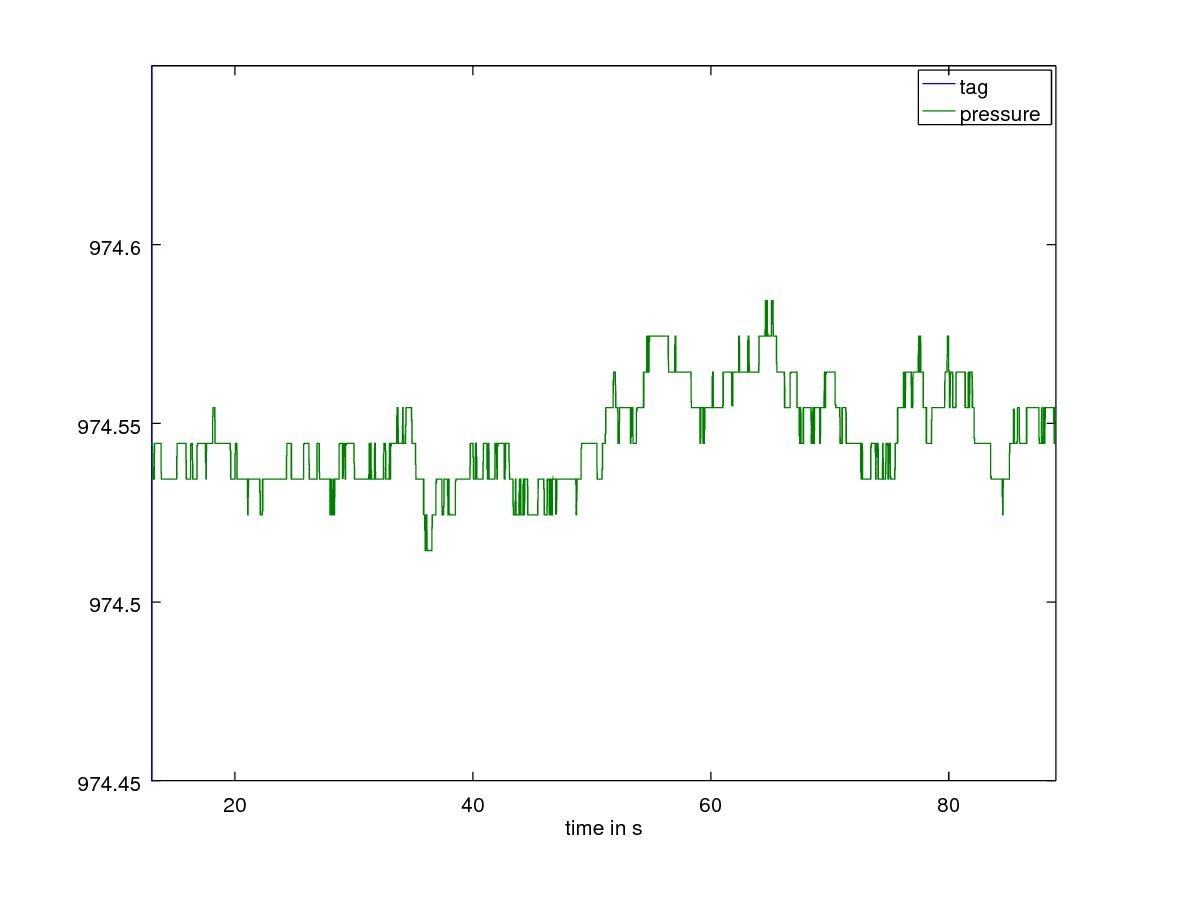
\includegraphics[width=.45\textwidth]{elevator4down1stop_still_p} &
		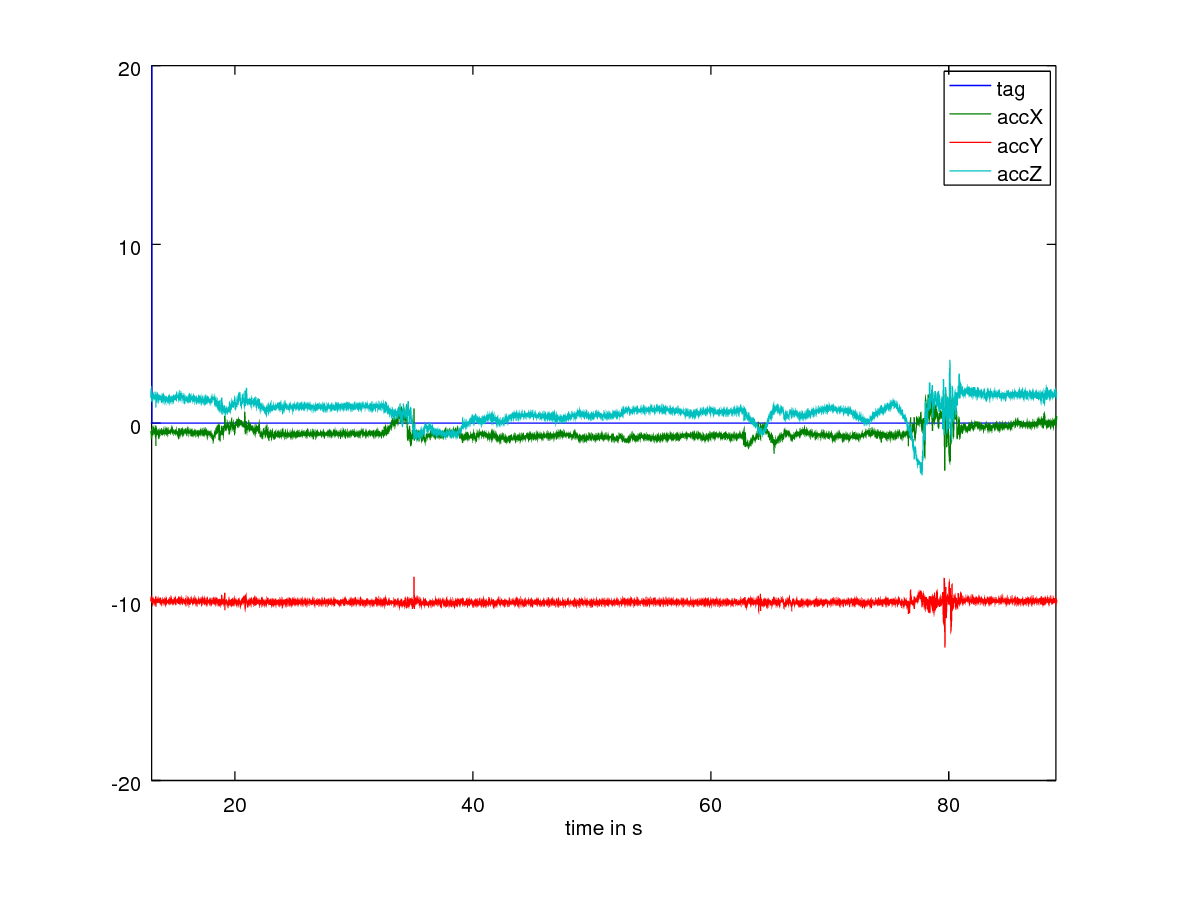
\includegraphics[width=.45\textwidth]{elevator4down1stop_still_a} 
		\\
		(a) & (b)
		\\[4pt]	%vertical extra spacing (4 points)
		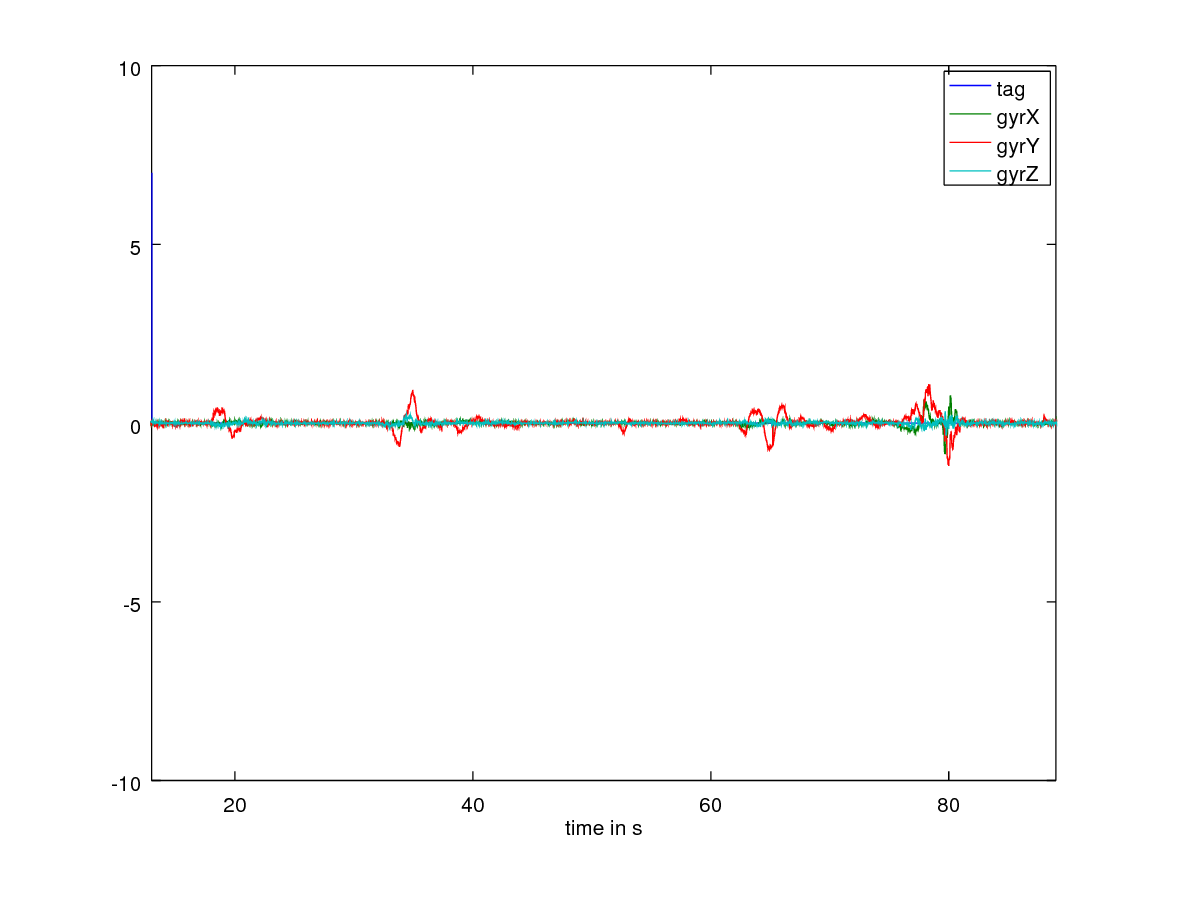
\includegraphics[width=.45\textwidth]{elevator4down1stop_still_g} &
		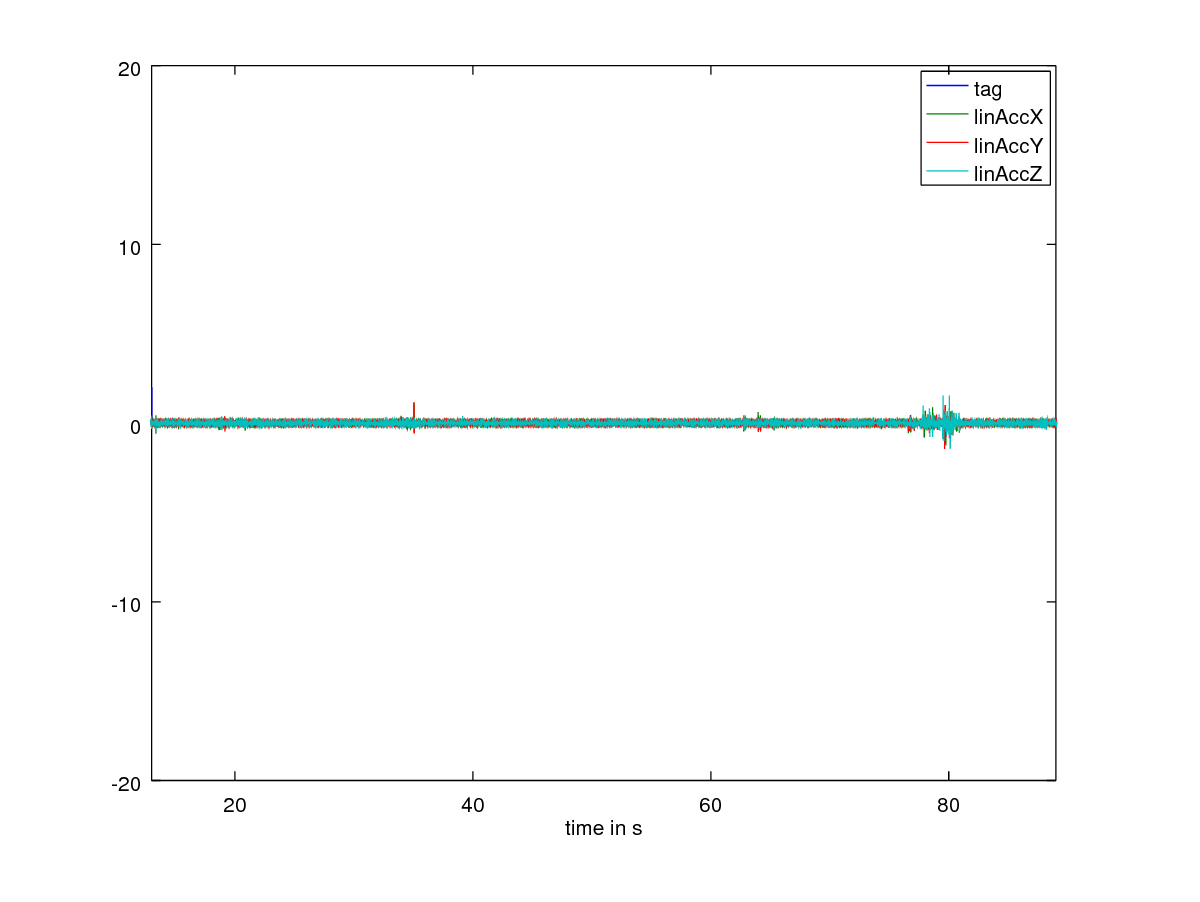
\includegraphics[width=.45\textwidth]{elevator4down1stop_still_la}
		\\
		(c) & (d)
		\\[4pt]	%vertical extra spacing (4 points)
		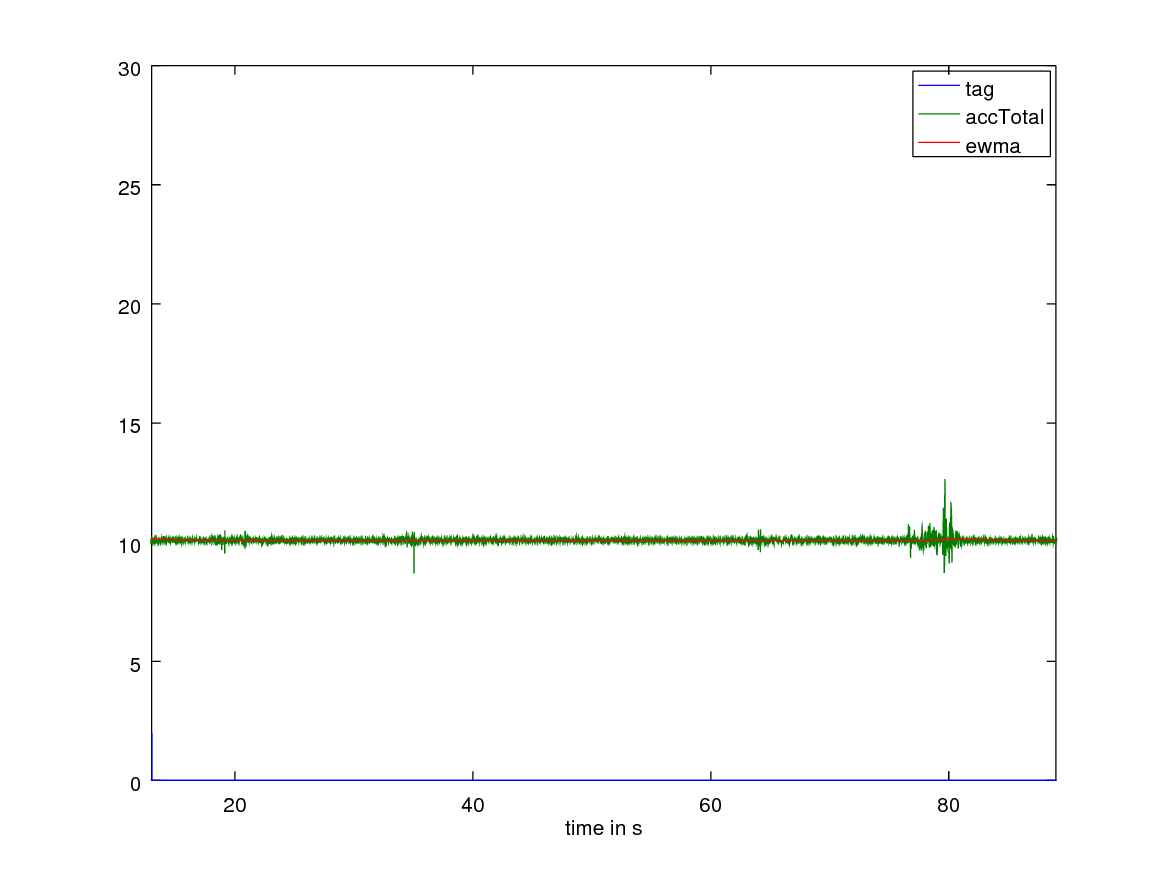
\includegraphics[width=.45\textwidth]{elevator4down1stop_still_atotal} &
		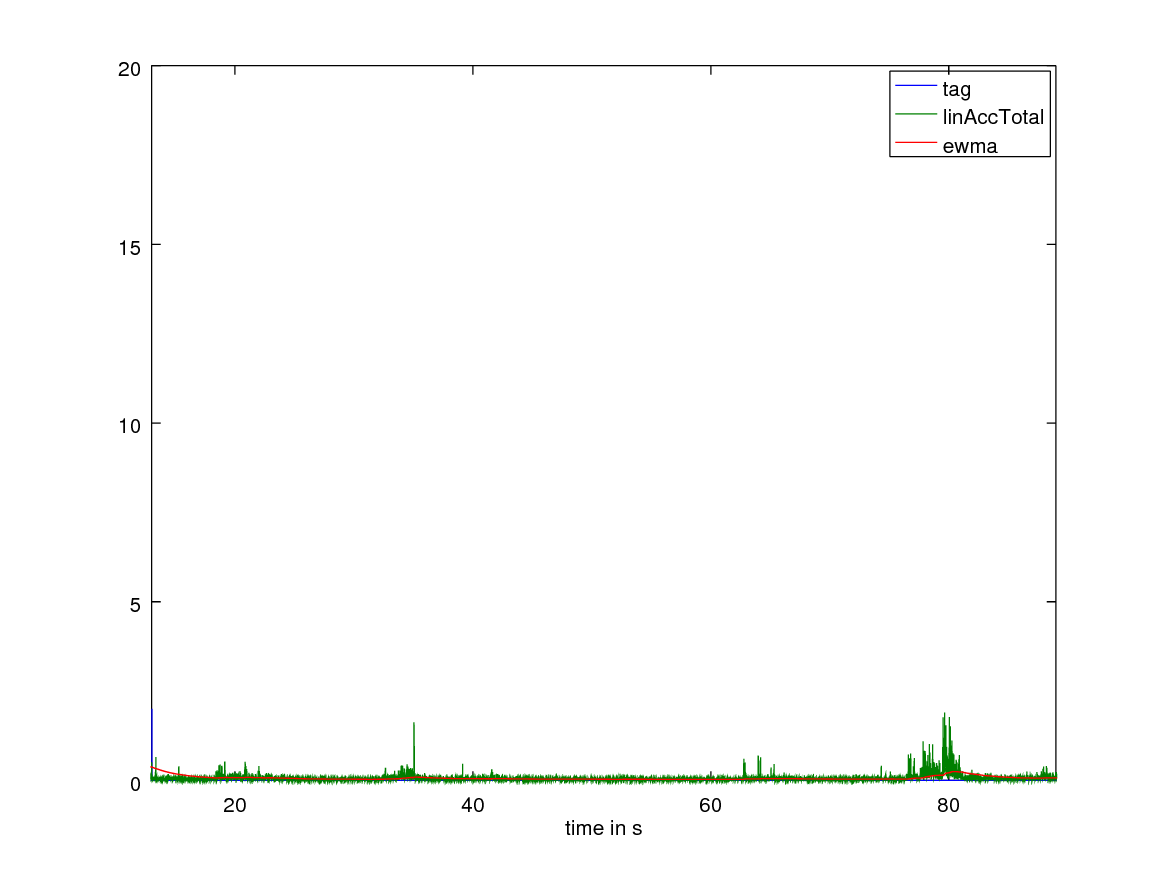
\includegraphics[width=.45\textwidth]{elevator4down1stop_still_latotal}
		\\
		(e) & (f)
	\end{tabular}
	%
	\caption{Test case 1}
	\label{fig:Test_case_still_1}
\end{figure}

%%%----------------------------------------------------------
\section{Test case 2}
%%%----------------------------------------------------------
Test case 2 in Fig.~\ref{fig:Test_case_still_2}
\begin{figure}
	\centering\small
	\setlength{\tabcolsep}{0mm}	% alle Spaltenränder auf 0mm
	\begin{tabular}{c@{\hspace{12mm}}c} % mittlerer Abstand = 12mm
		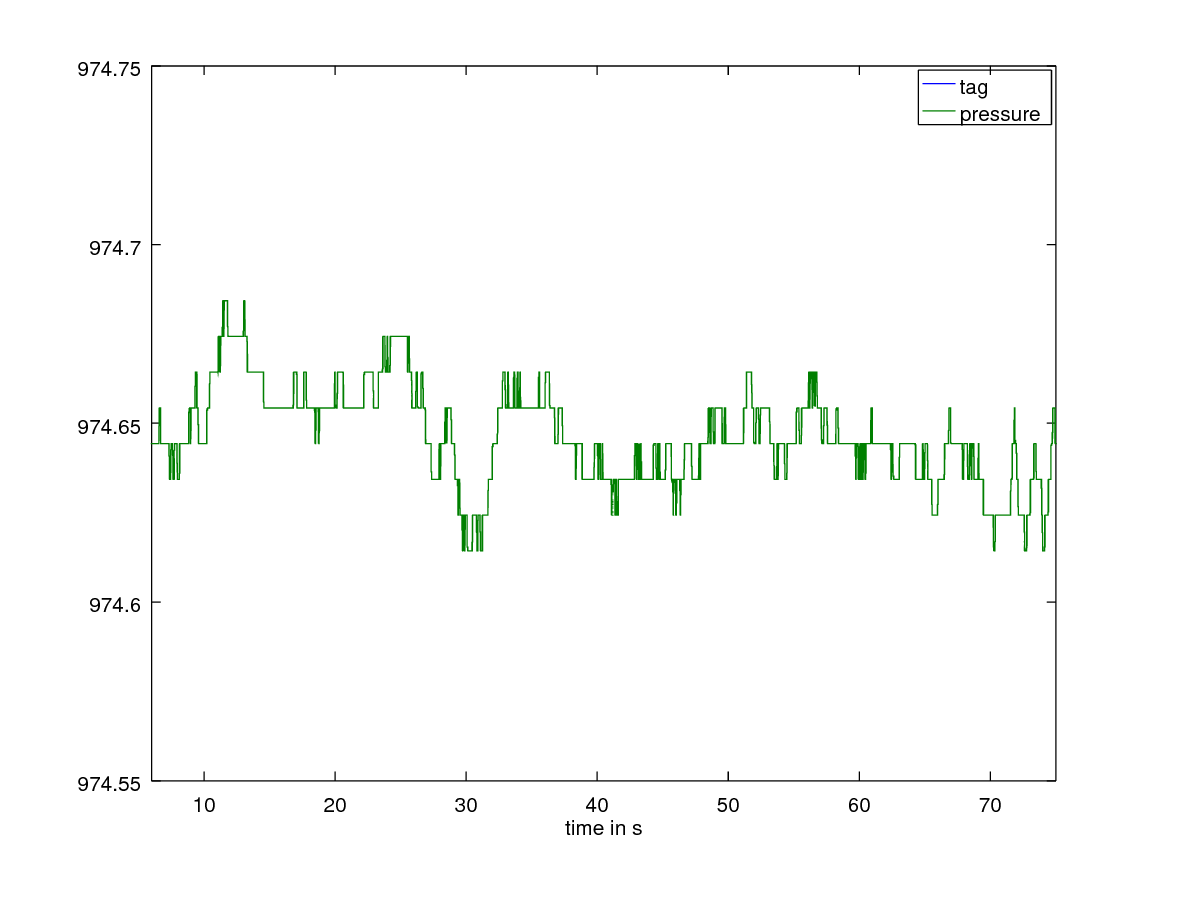
\includegraphics[width=.45\textwidth]{elevator4down2stops_still_p} &
		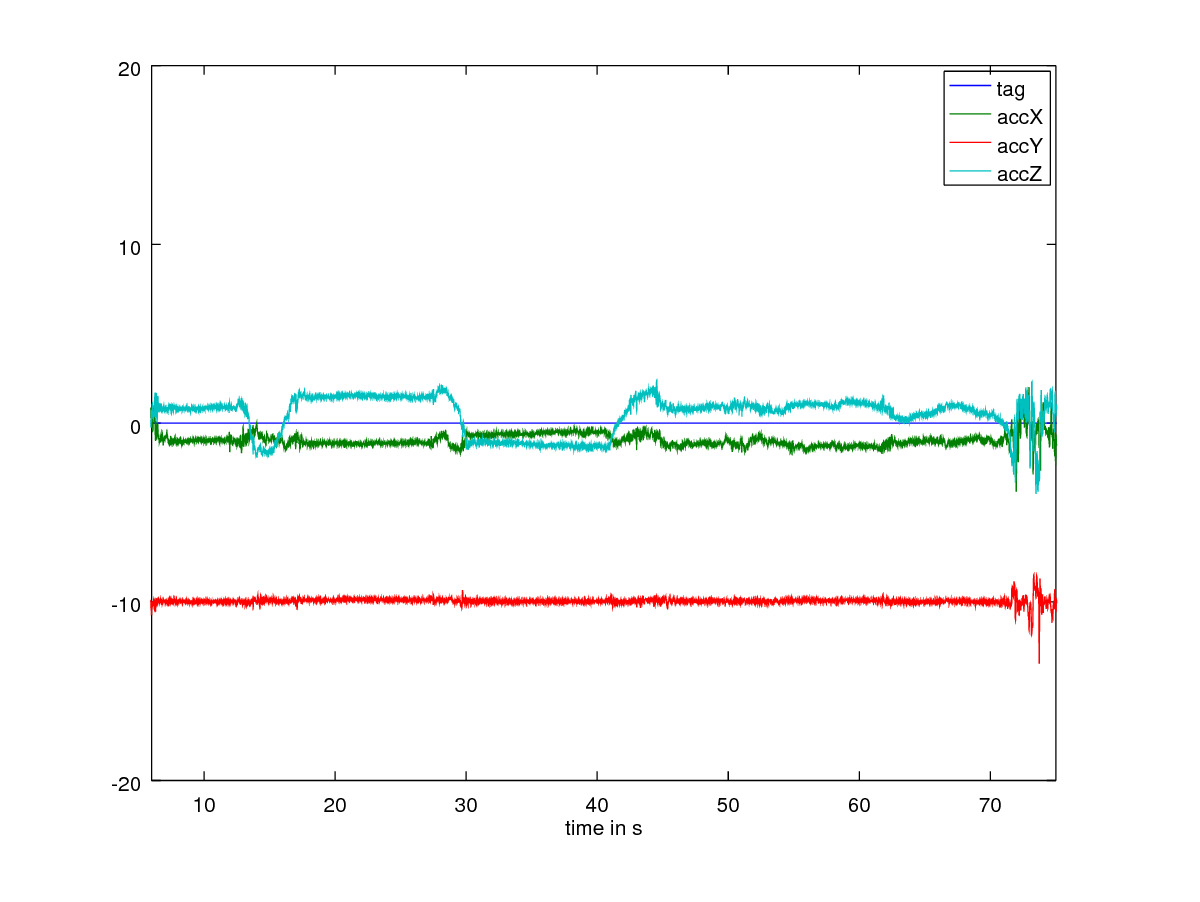
\includegraphics[width=.45\textwidth]{elevator4down2stops_still_a} 
		\\
		(a) & (b)
		\\[4pt]	%vertical extra spacing (4 points)
		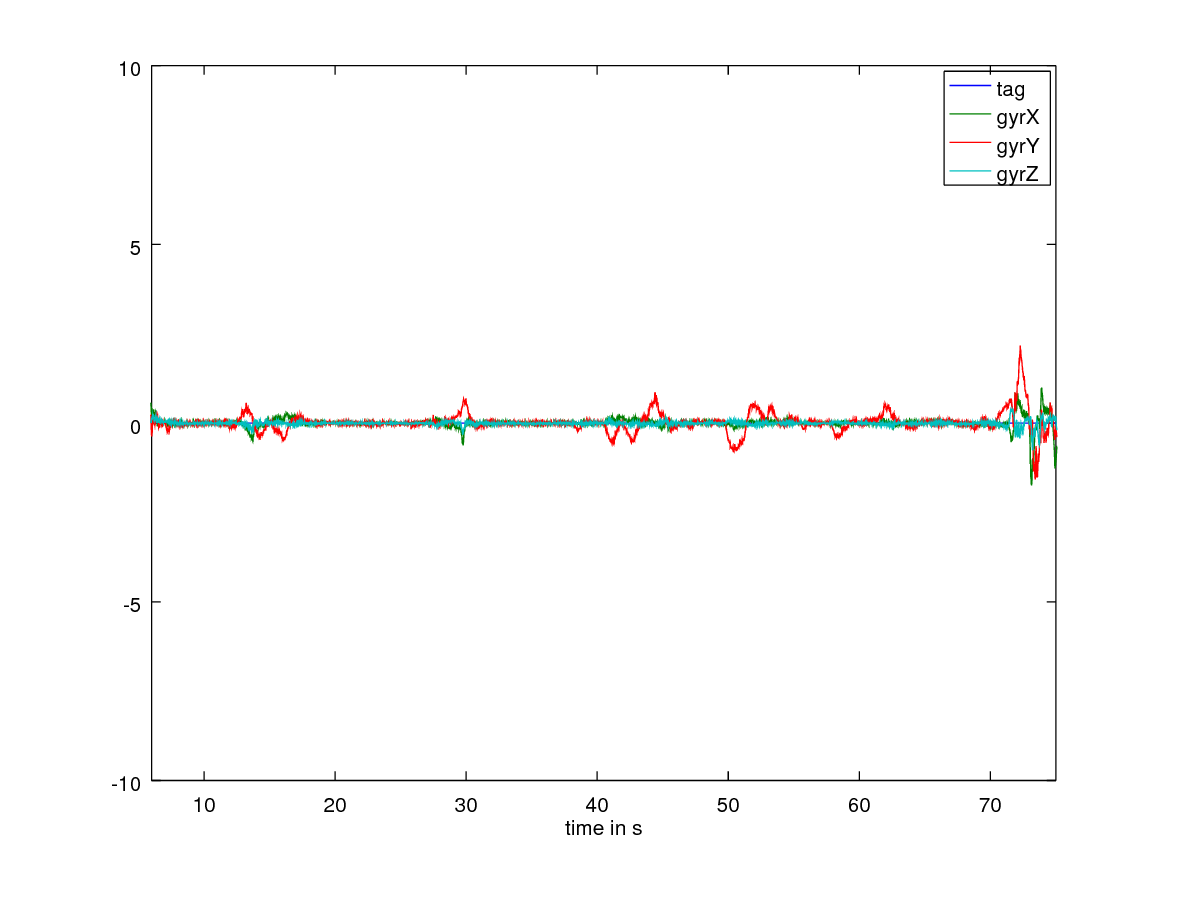
\includegraphics[width=.45\textwidth]{elevator4down2stops_still_g} &
		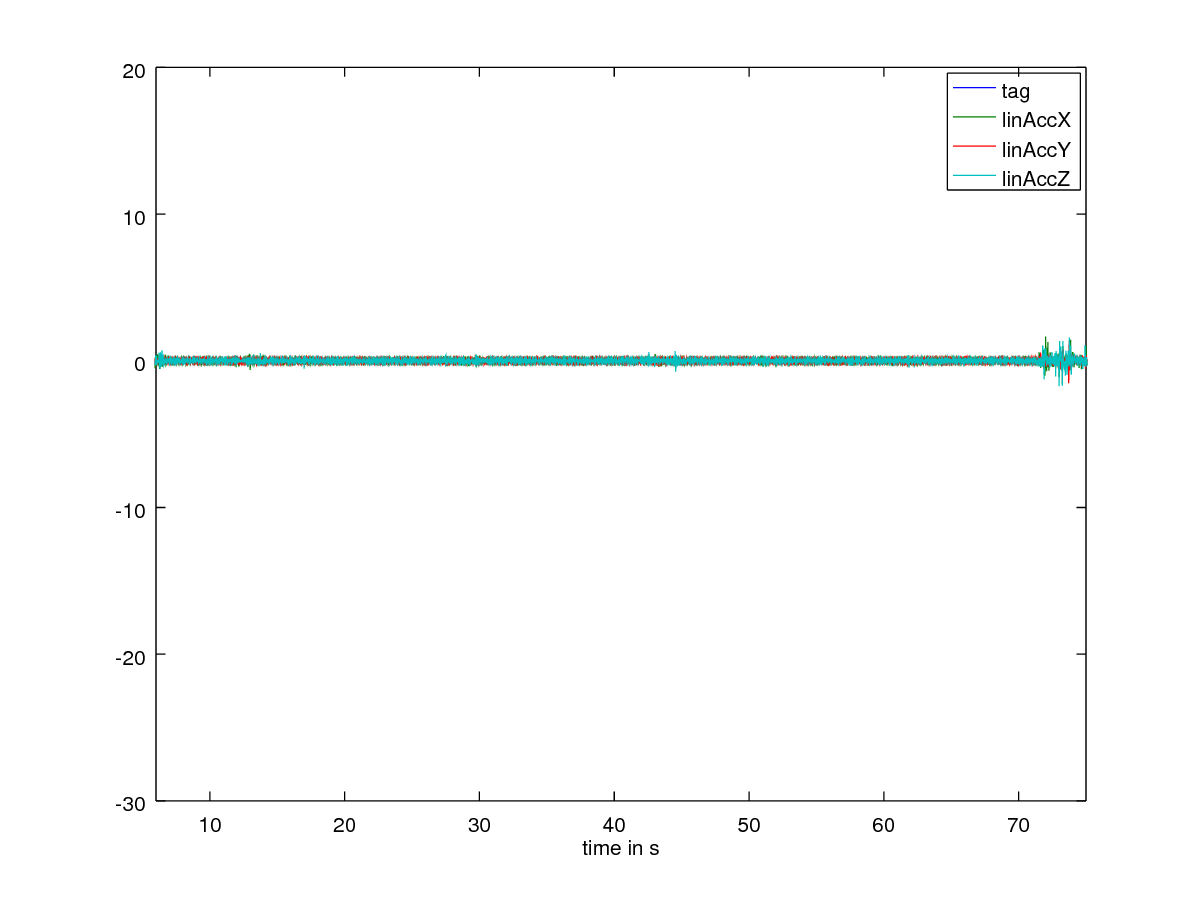
\includegraphics[width=.45\textwidth]{elevator4down2stops_still_la}
		\\
		(c) & (d)
		\\[4pt]	%vertical extra spacing (4 points)
		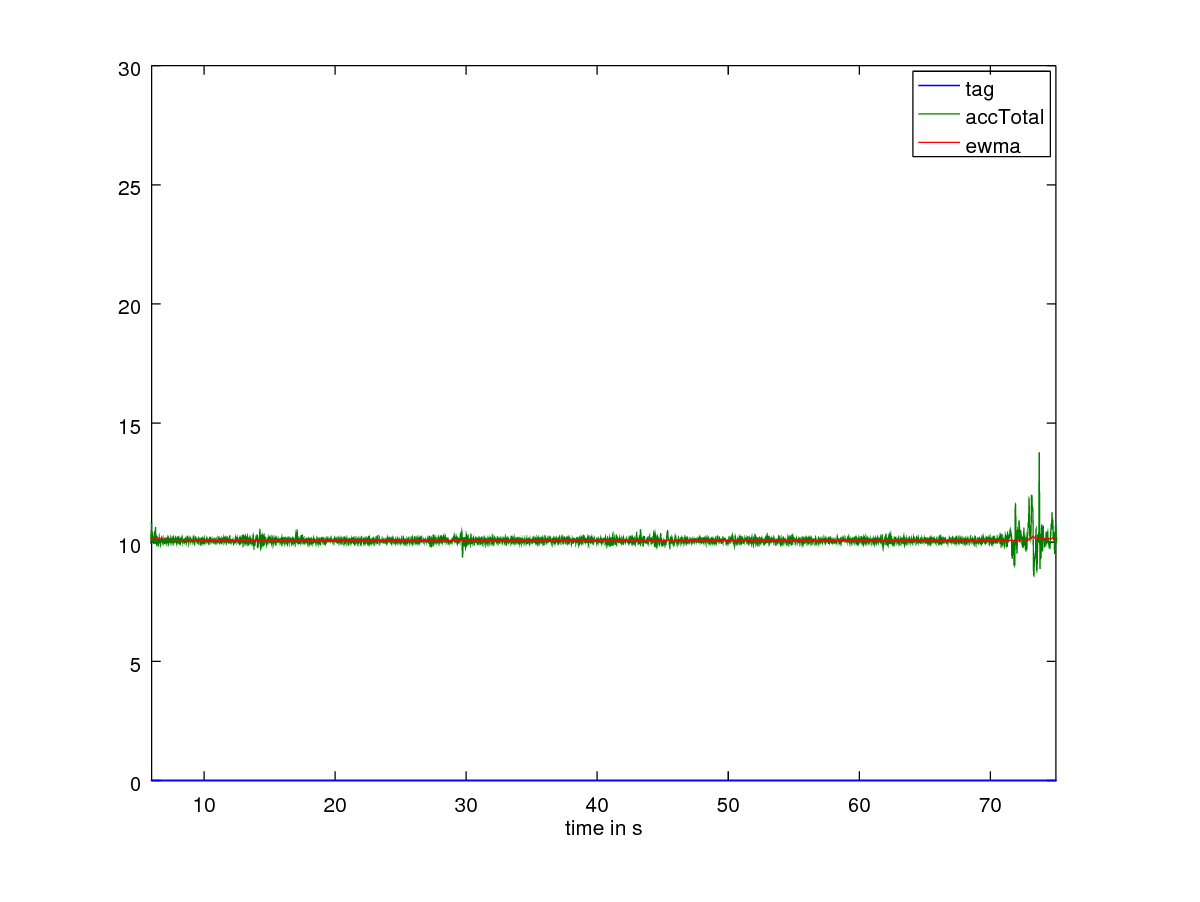
\includegraphics[width=.45\textwidth]{elevator4down2stops_still_atotal} &
		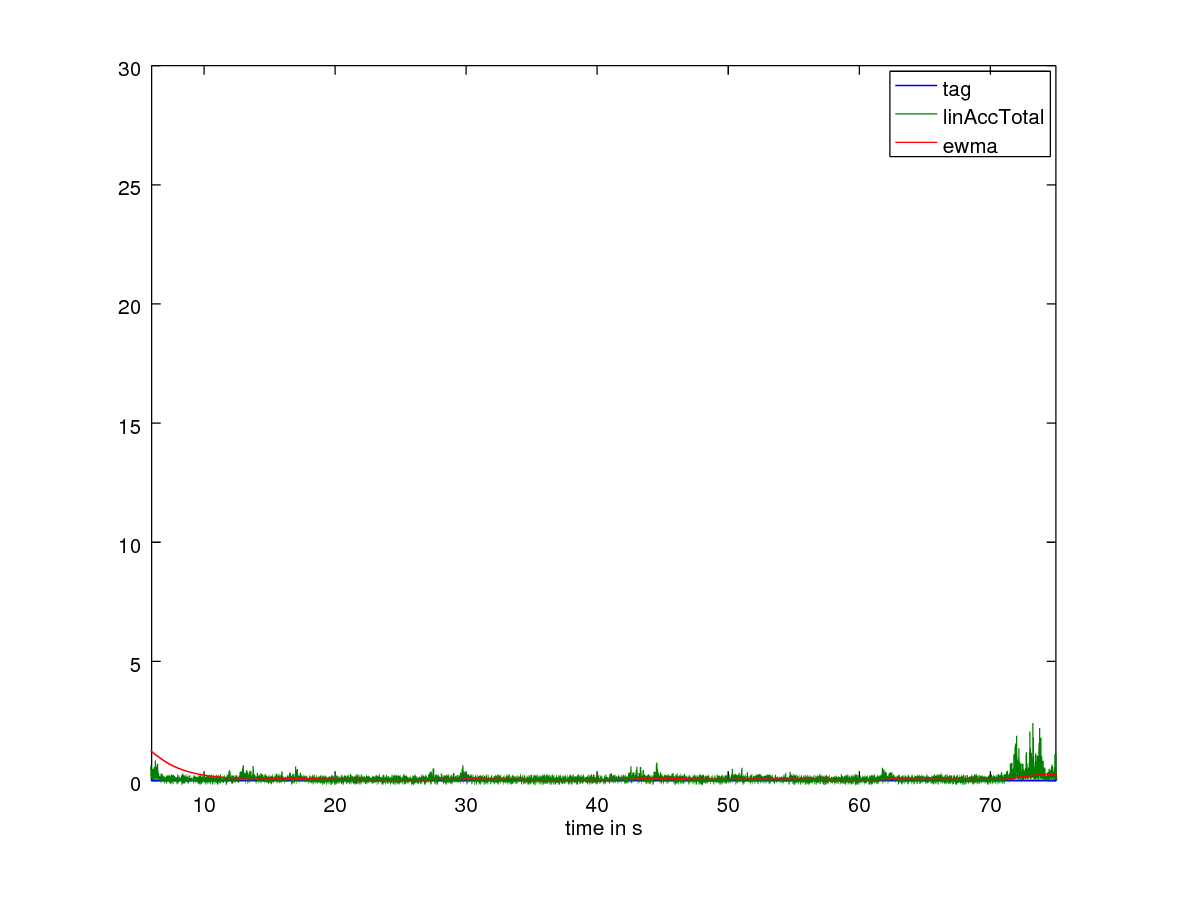
\includegraphics[width=.45\textwidth]{elevator4down2stops_still_latotal}
		\\
		(e) & (f)
	\end{tabular}
	%
	\caption{Test case 2}
	\label{fig:Test_case_still_2}
\end{figure}

%%%----------------------------------------------------------
\section{Test case 3}
%%%----------------------------------------------------------
Test case 3 in Fig.~\ref{fig:Test_case_still_3}
\begin{figure}
	\centering\small
	\setlength{\tabcolsep}{0mm}	% alle Spaltenränder auf 0mm
	\begin{tabular}{c@{\hspace{12mm}}c} % mittlerer Abstand = 12mm
			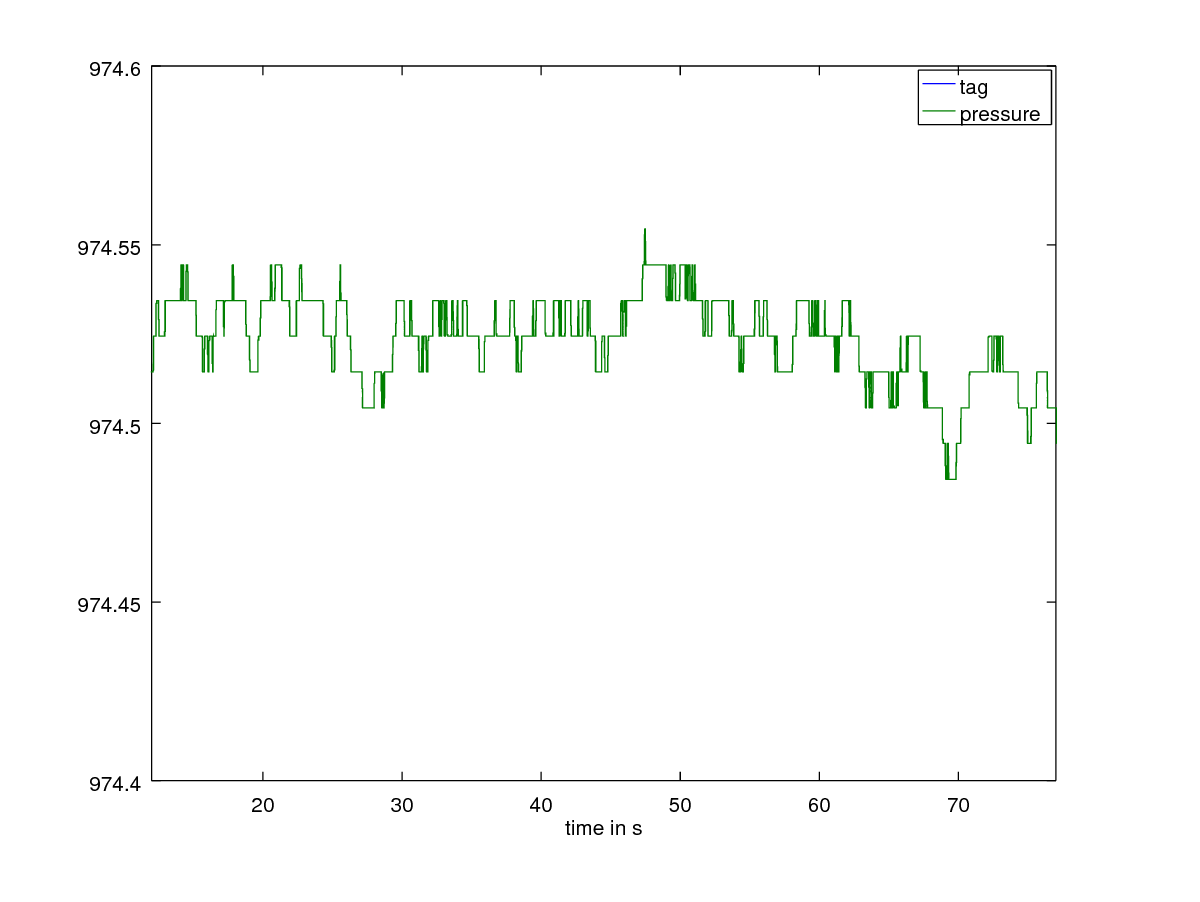
\includegraphics[width=.45\textwidth]{elevator5down1stop_still_p} &
			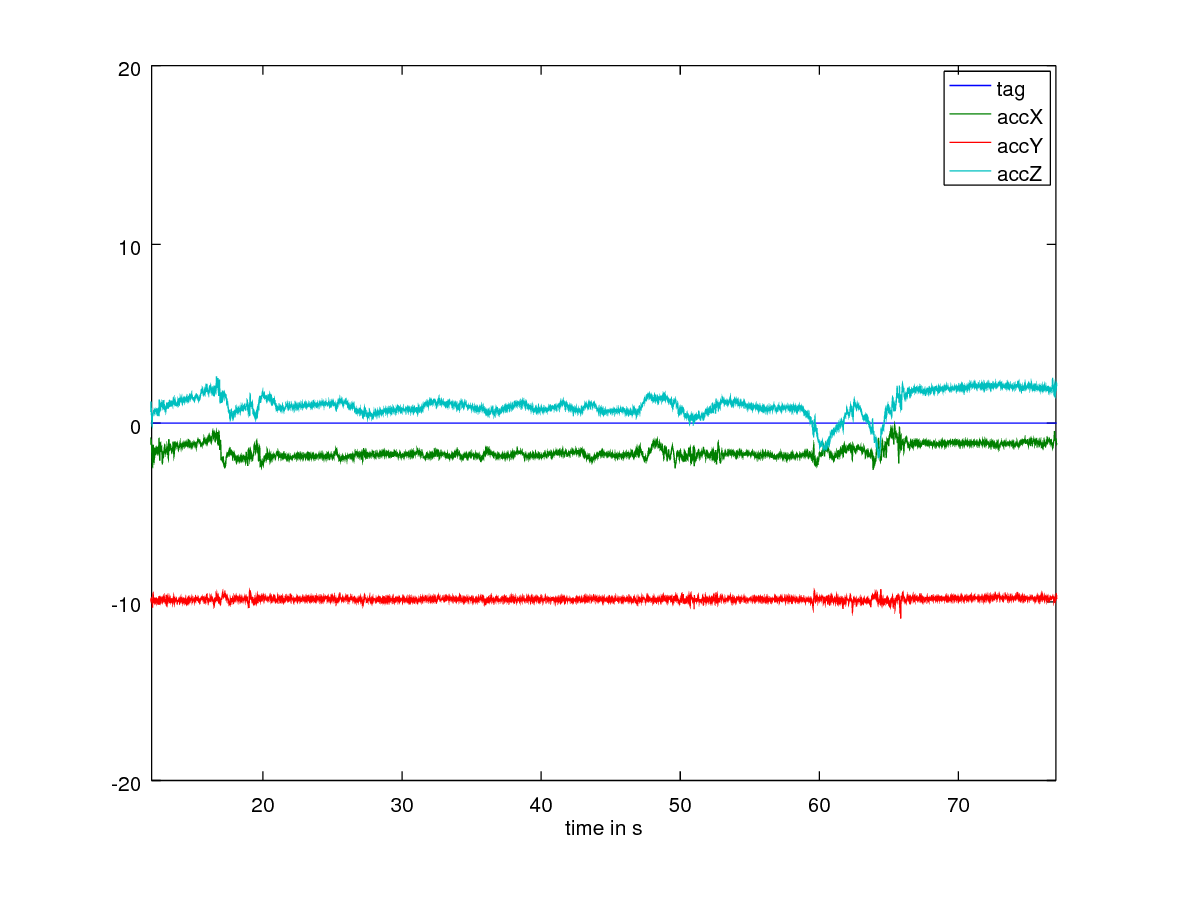
\includegraphics[width=.45\textwidth]{elevator5down1stop_still_a} 
			\\
			(a) & (b)
			\\[4pt]	%vertical extra spacing (4 points)
			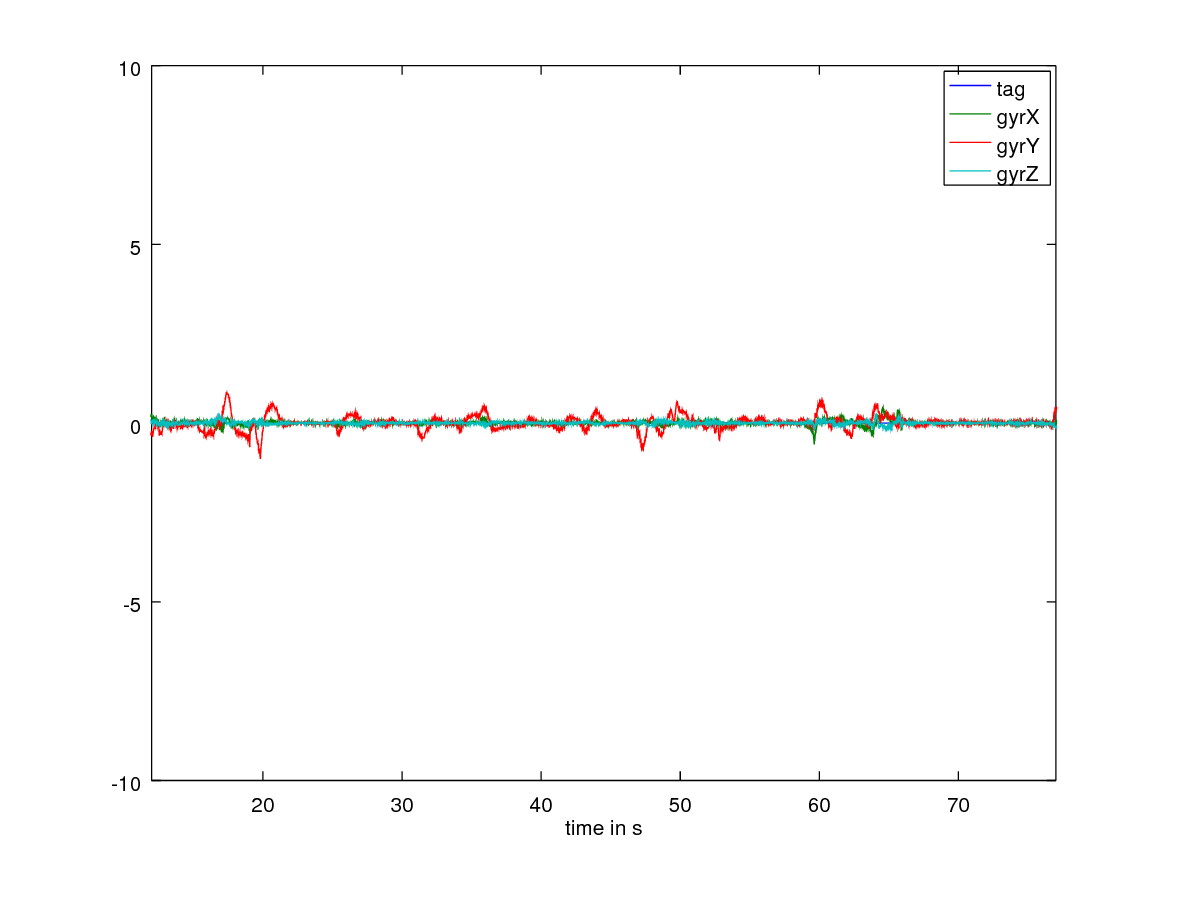
\includegraphics[width=.45\textwidth]{elevator5down1stop_still_g} &
			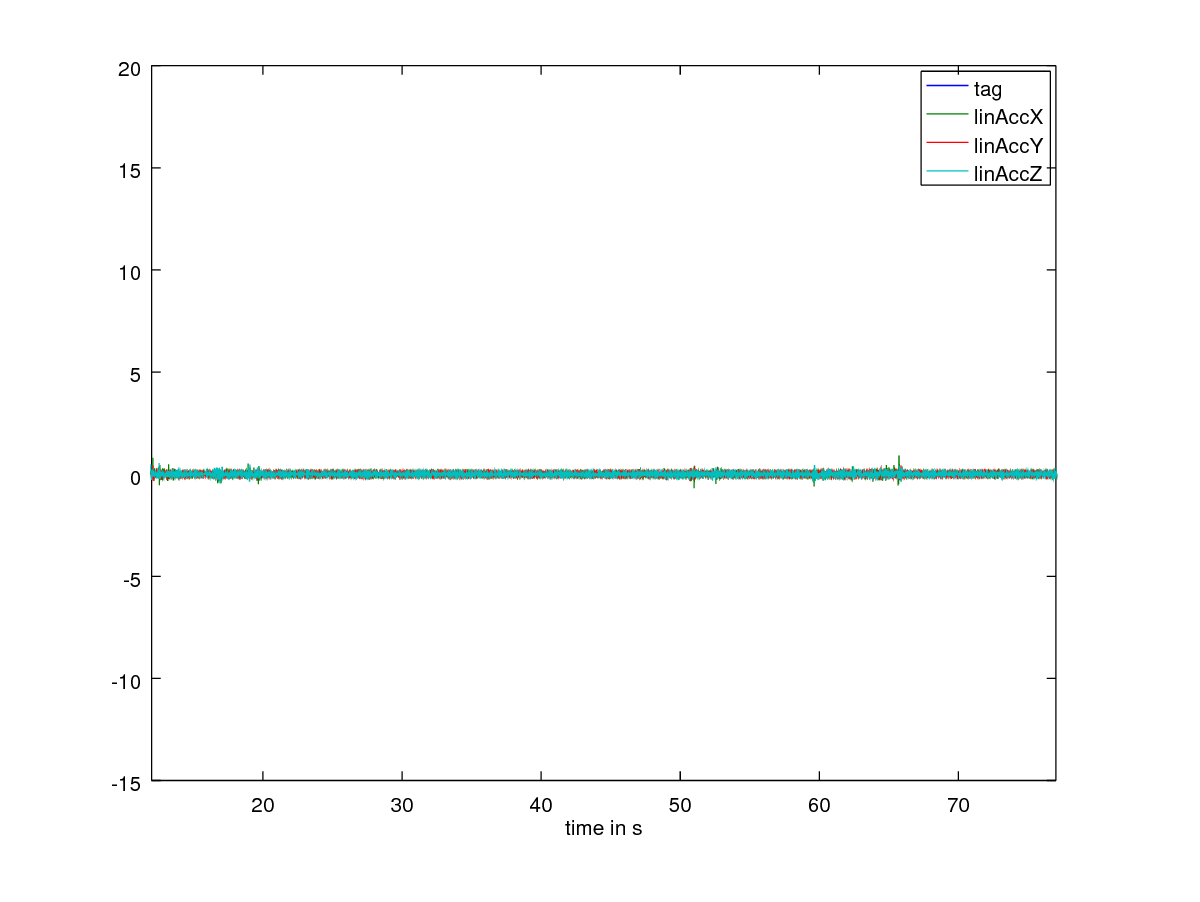
\includegraphics[width=.45\textwidth]{elevator5down1stop_still_la}
			\\
			(c) & (d)
			\\[4pt]	%vertical extra spacing (4 points)
			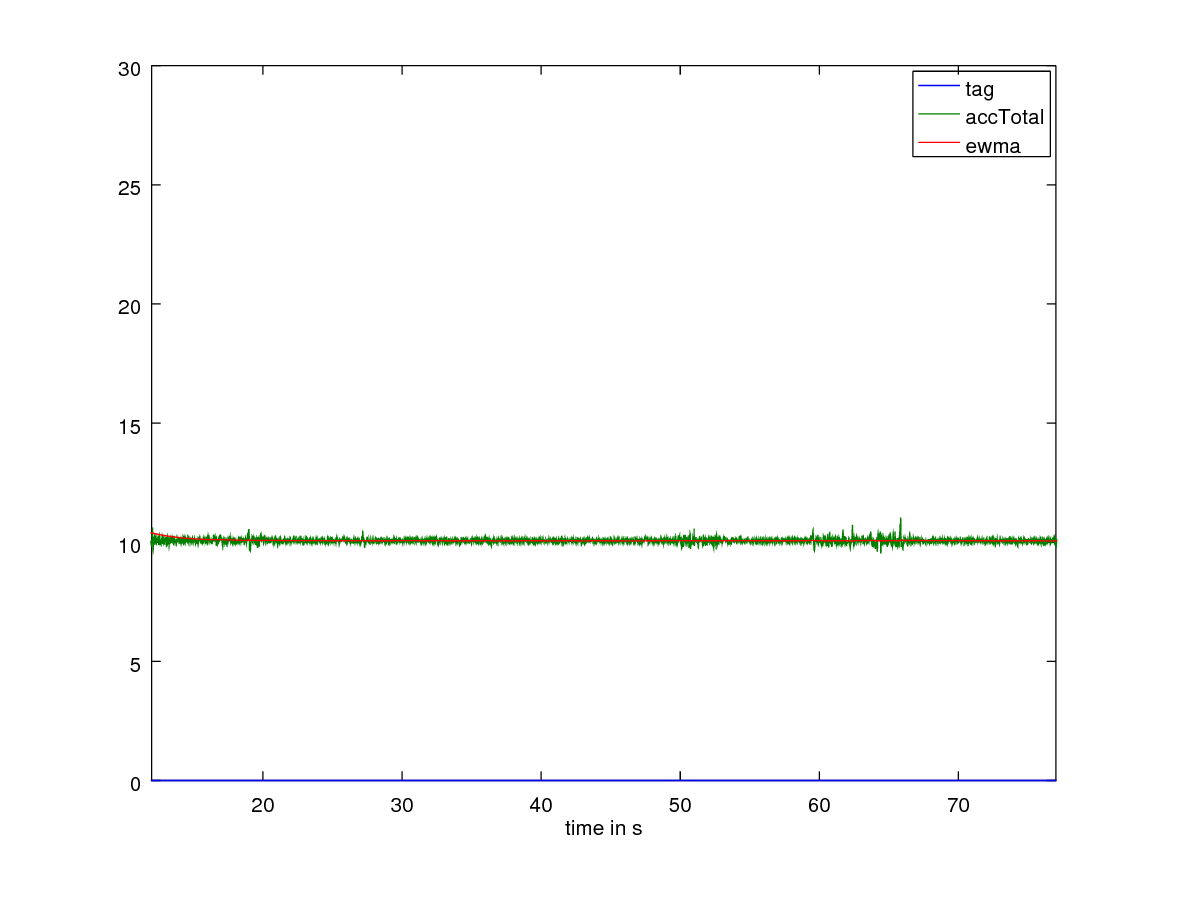
\includegraphics[width=.45\textwidth]{elevator5down1stop_still_atotal} &
			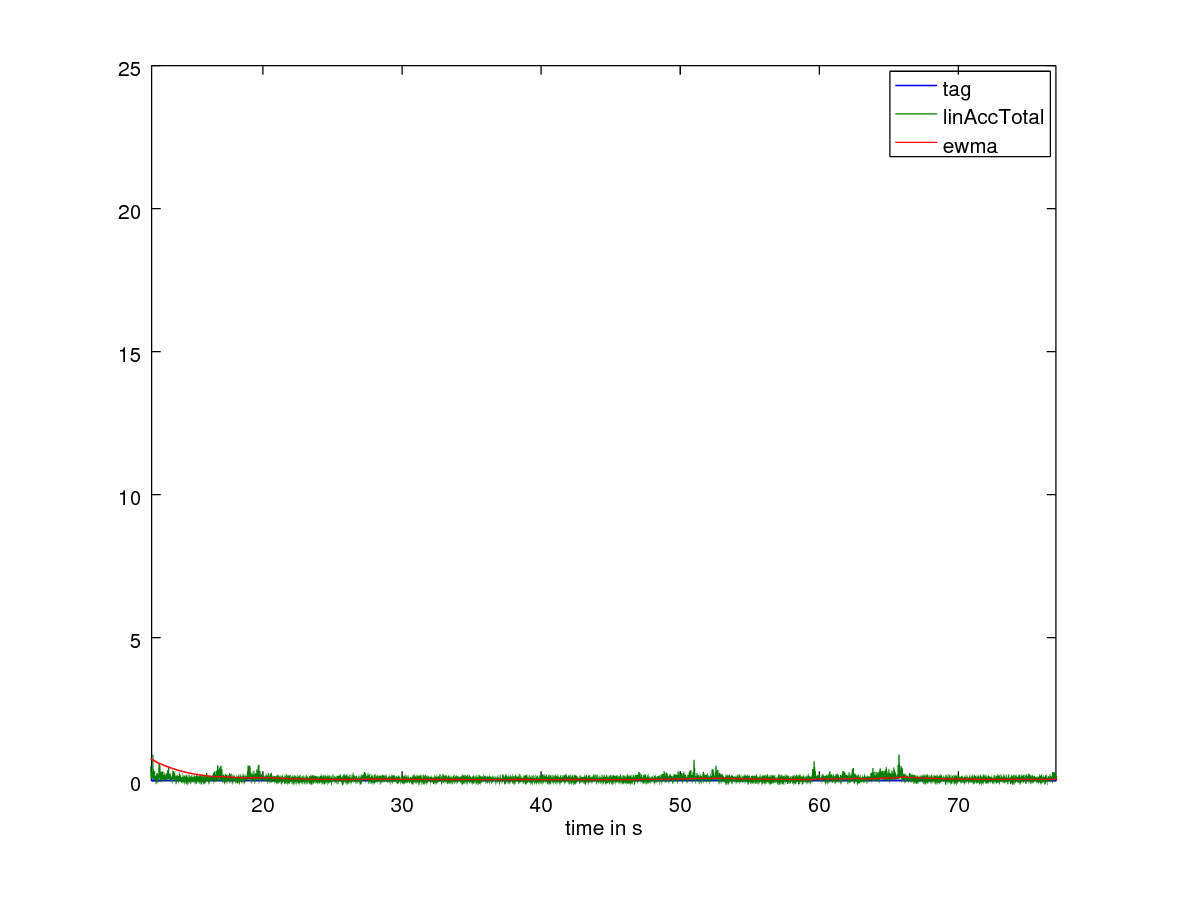
\includegraphics[width=.45\textwidth]{elevator5down1stop_still_latotal}
			\\
			(e) & (f)
	\end{tabular}
	%
	\caption{Test case 3}
	\label{fig:Test_case_still_3}
\end{figure}



%%%----------------------------------------------------------
%%%----------------------------------------------------------
%%%----------------------------------------------------------
%%%----------------------------------------------------------
%%%----------------------------------------------------------
\chapter{Walking}
%%%----------------------------------------------------------

The activity "walking" will be analyzed here with graphics.
%%%----------------------------------------------------------
\section{Test case 1}
%%%----------------------------------------------------------
Test case 1 in Fig.~\ref{fig:Test_case_1_walking}
\begin{figure}
	\centering\small
	\setlength{\tabcolsep}{0mm}	% alle Spaltenränder auf 0mm
	\begin{tabular}{c@{\hspace{12mm}}c} % mittlerer Abstand = 12mm
		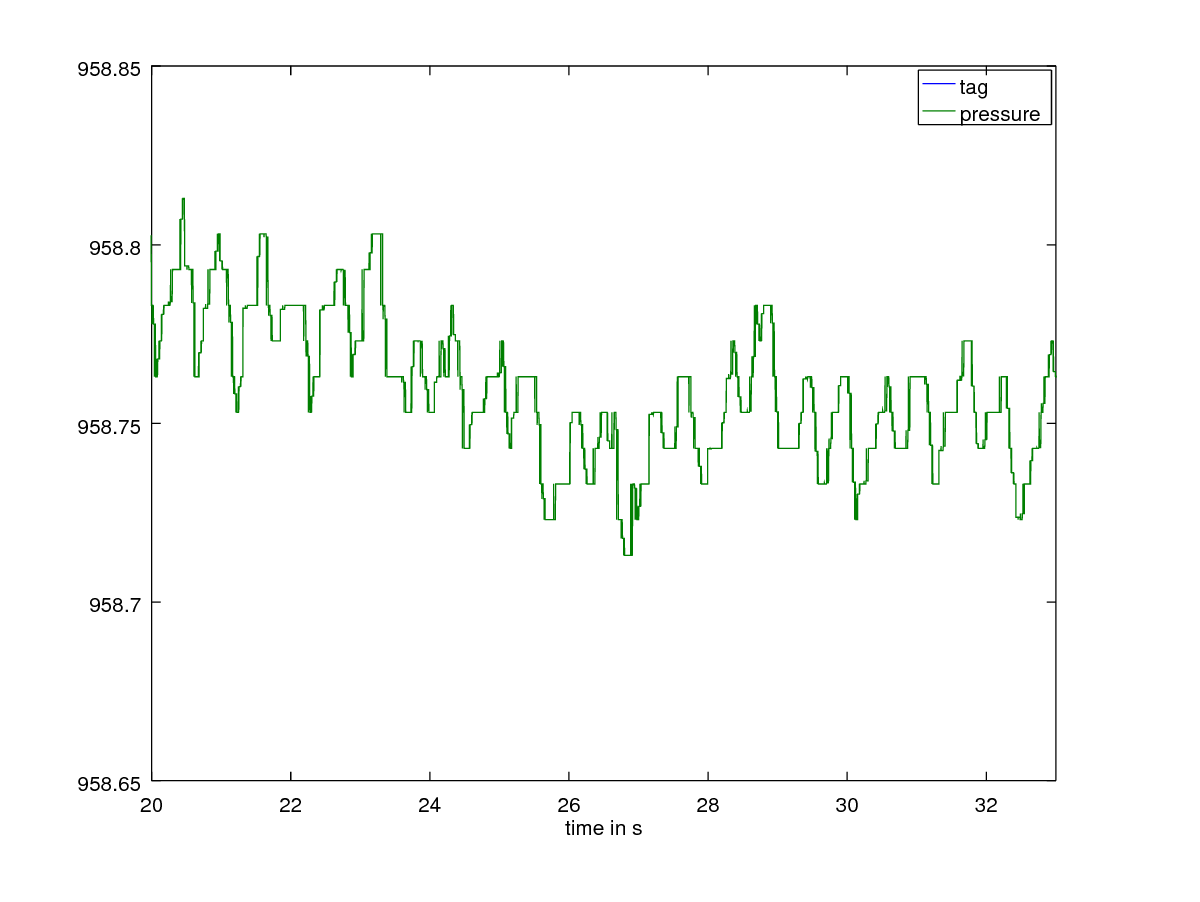
\includegraphics[width=.45\textwidth]{stairsfhdown_walking_p} &
		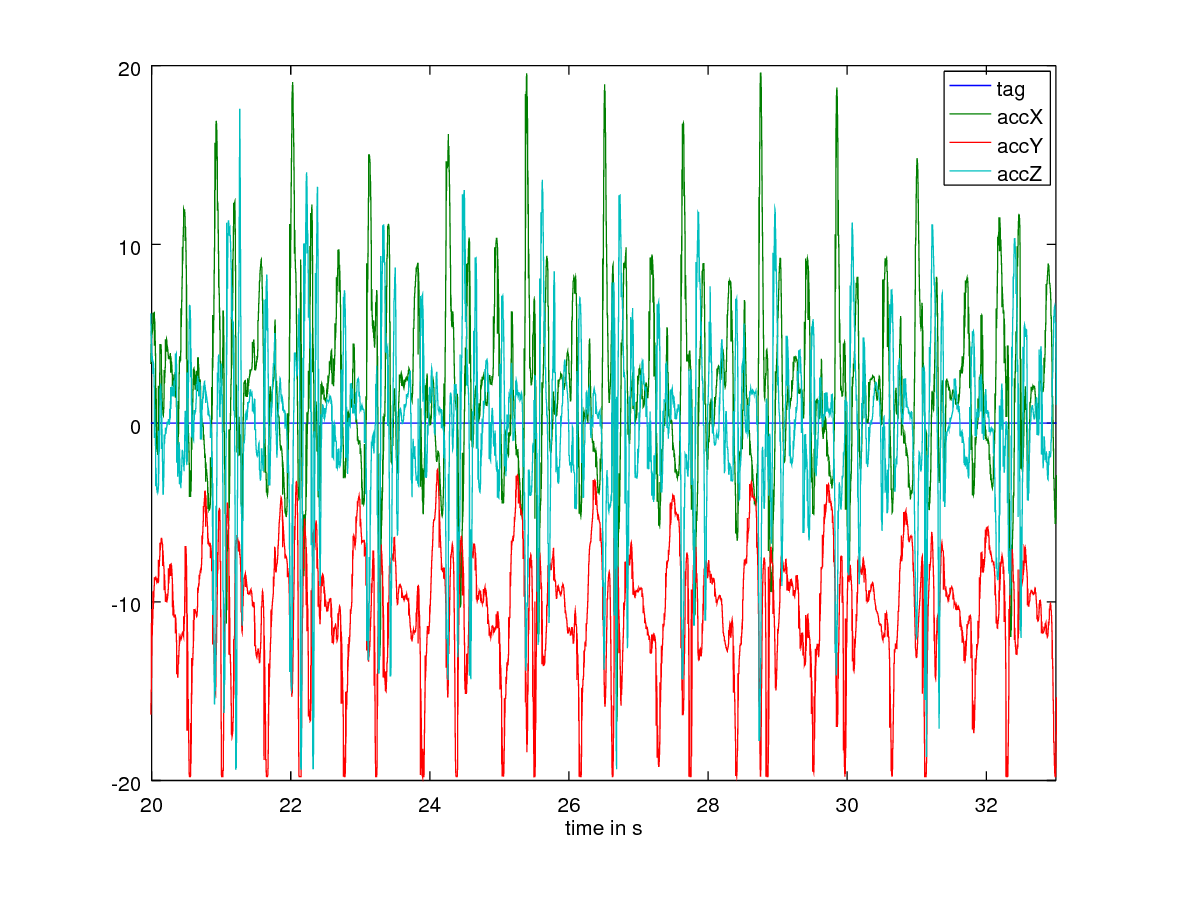
\includegraphics[width=.45\textwidth]{stairsfhdown_walking_a} 
		\\
		(a) & (b)
		\\[4pt]	%vertical extra spacing (4 points)
		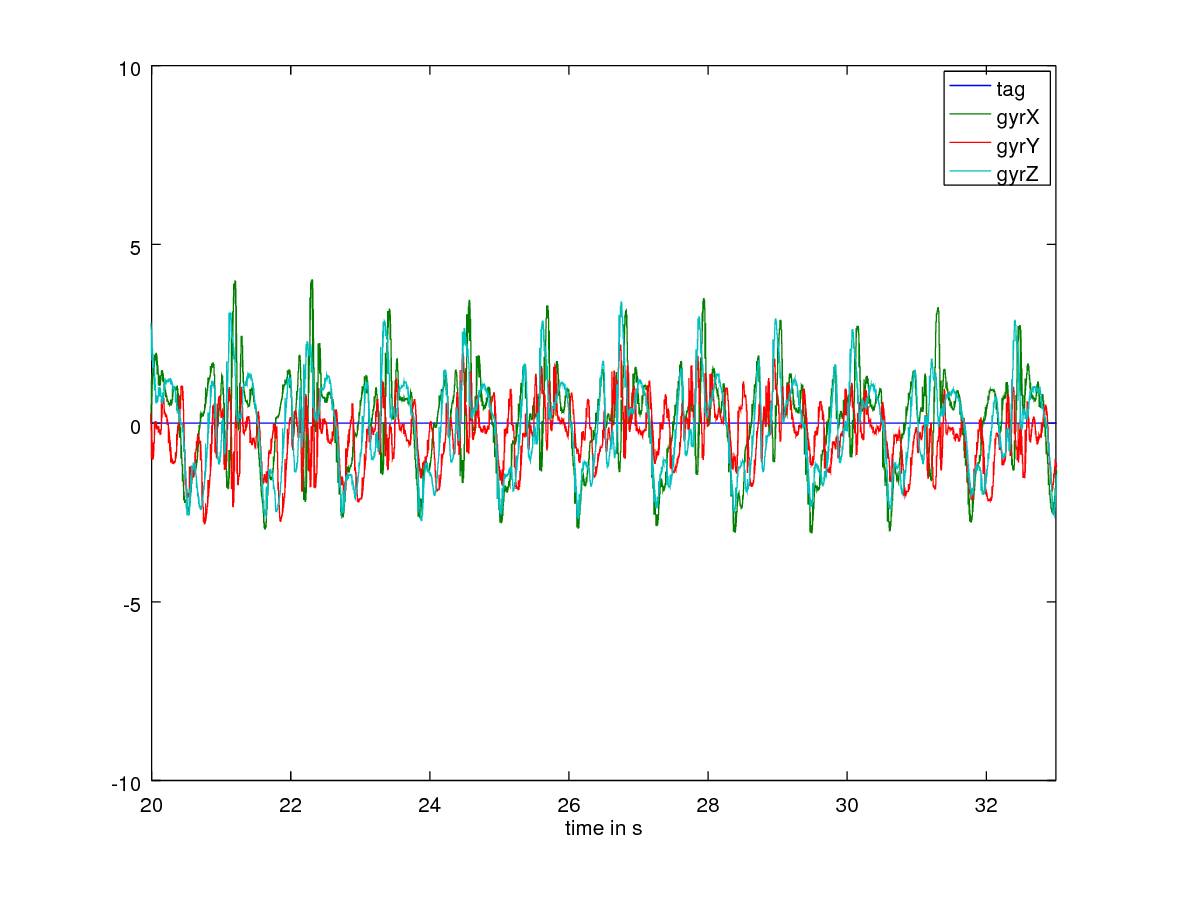
\includegraphics[width=.45\textwidth]{stairsfhdown_walking_g} &
		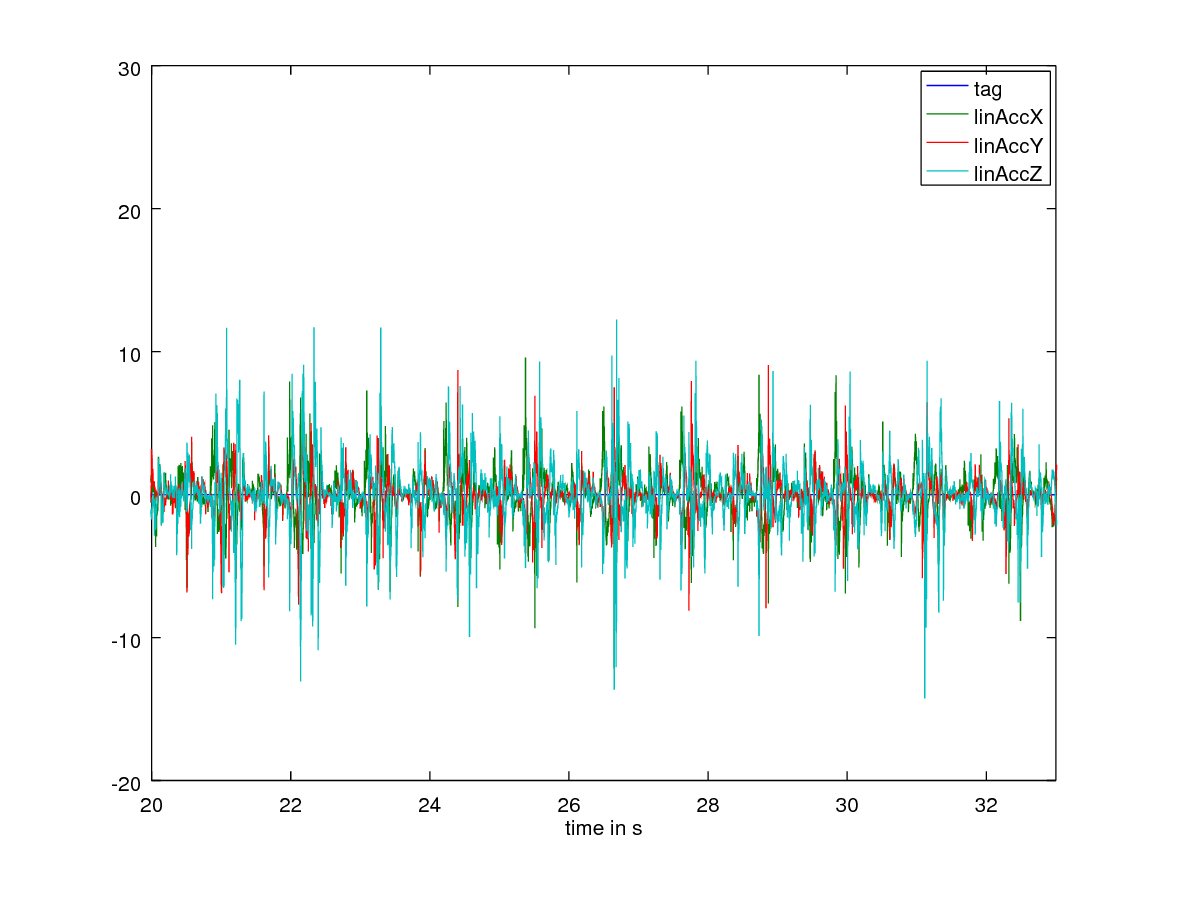
\includegraphics[width=.45\textwidth]{stairsfhdown_walking_la} 
		\\
		(c) & (d)
		\\[4pt]	%vertical extra spacing (4 points)
		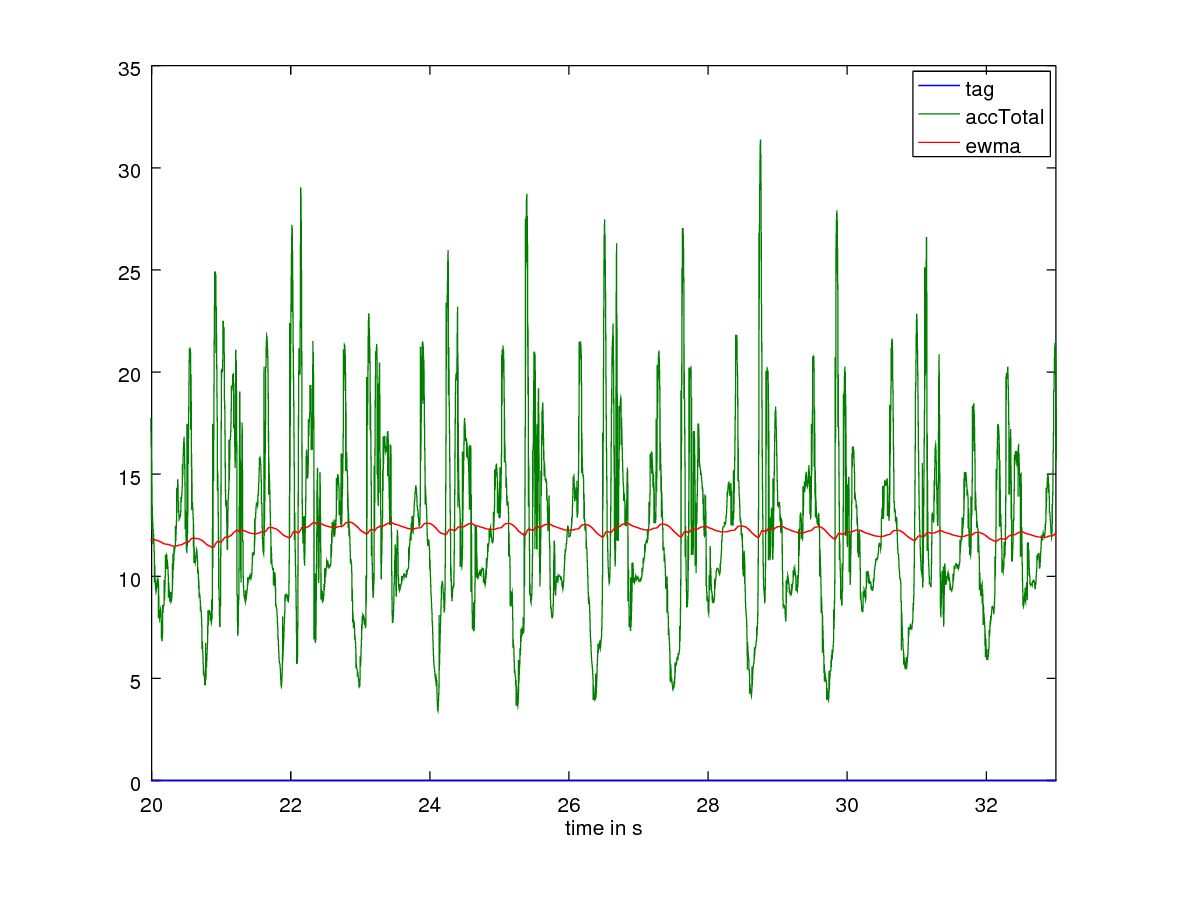
\includegraphics[width=.45\textwidth]{stairsfhdown_walking_atotal} &
		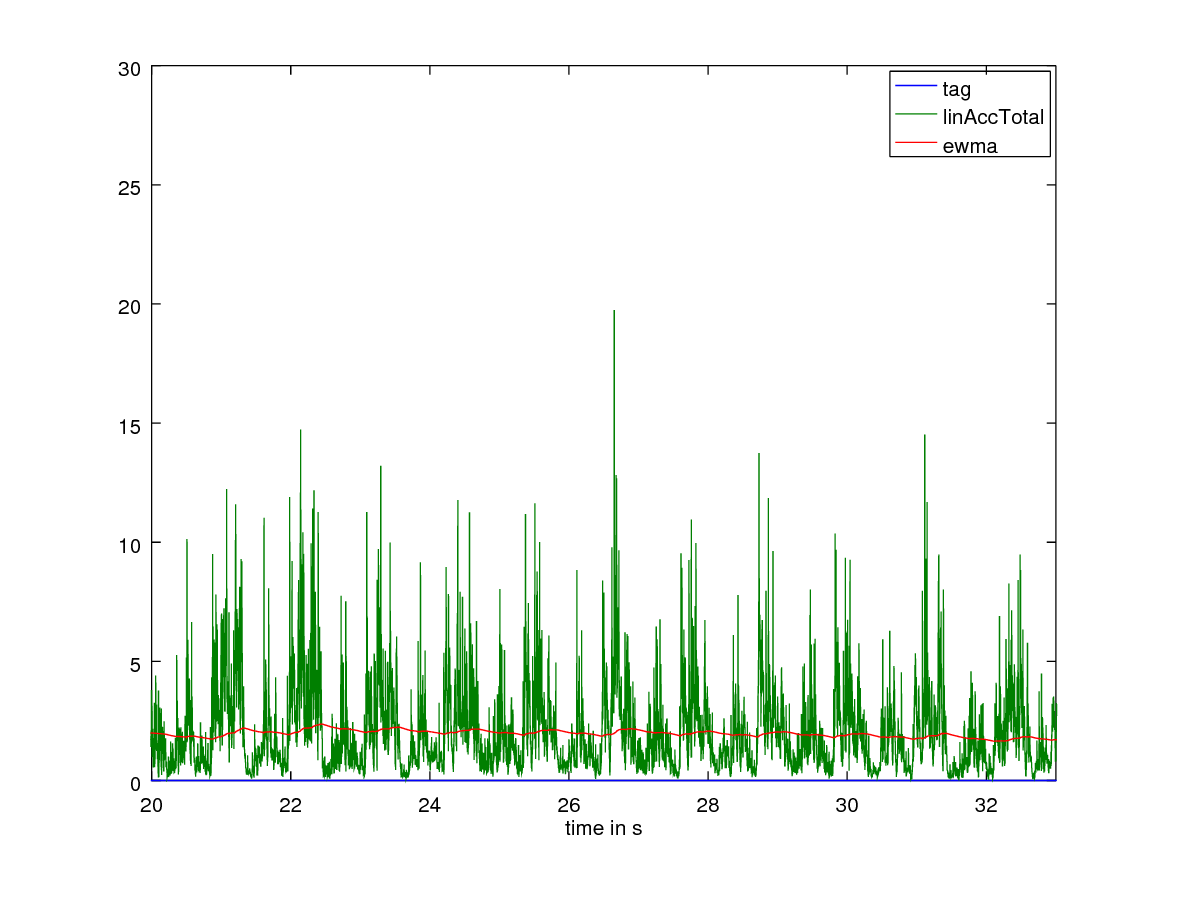
\includegraphics[width=.45\textwidth]{stairsfhdown_walking_latotal} 
		\\
		(e) & (f)
	\end{tabular}
	%
	\caption{Test case 1}
	\label{fig:Test_case_1_walking}
\end{figure}

%%%----------------------------------------------------------
\section{Test case 2}
%%%----------------------------------------------------------

Test case 2 in Fig.~\ref{fig:Test_case_2_walking}
\begin{figure}
	\centering\small
	\setlength{\tabcolsep}{0mm}	% alle Spaltenränder auf 0mm
	\begin{tabular}{c@{\hspace{12mm}}c} % mittlerer Abstand = 12mm
	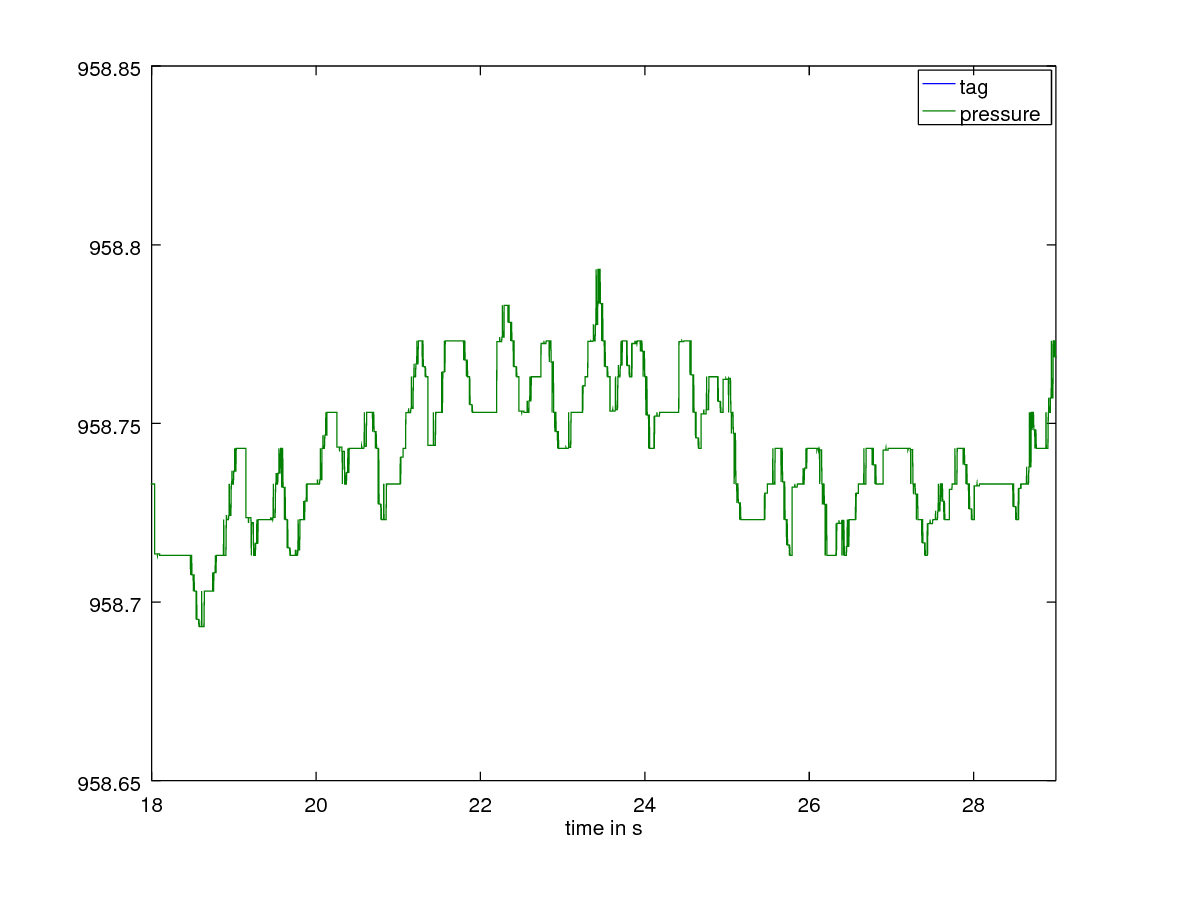
\includegraphics[width=.45\textwidth]{stairsfhdown2_walking_p} &
	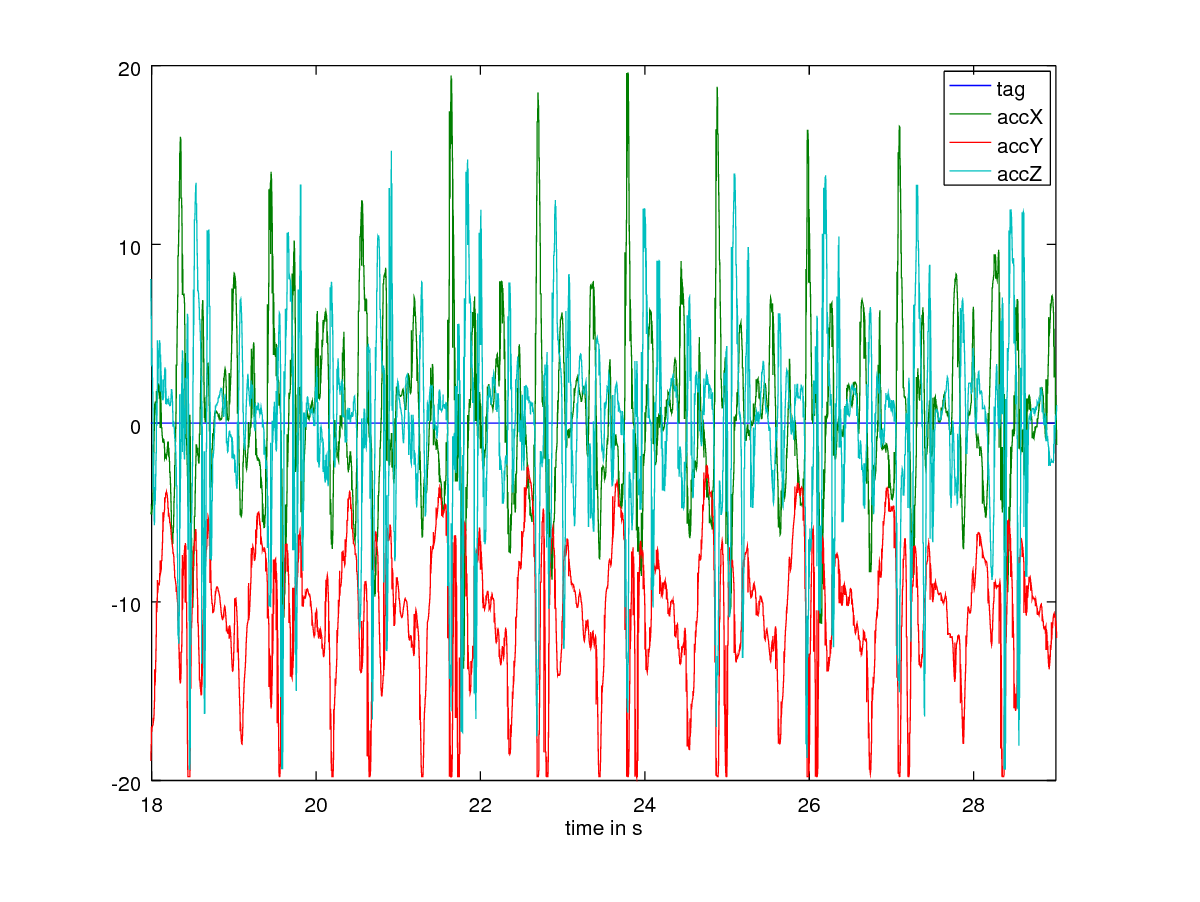
\includegraphics[width=.45\textwidth]{stairsfhdown2_walking_a} 
	\\
	(a) & (b)
	\\[4pt]	%vertical extra spacing (4 points)
	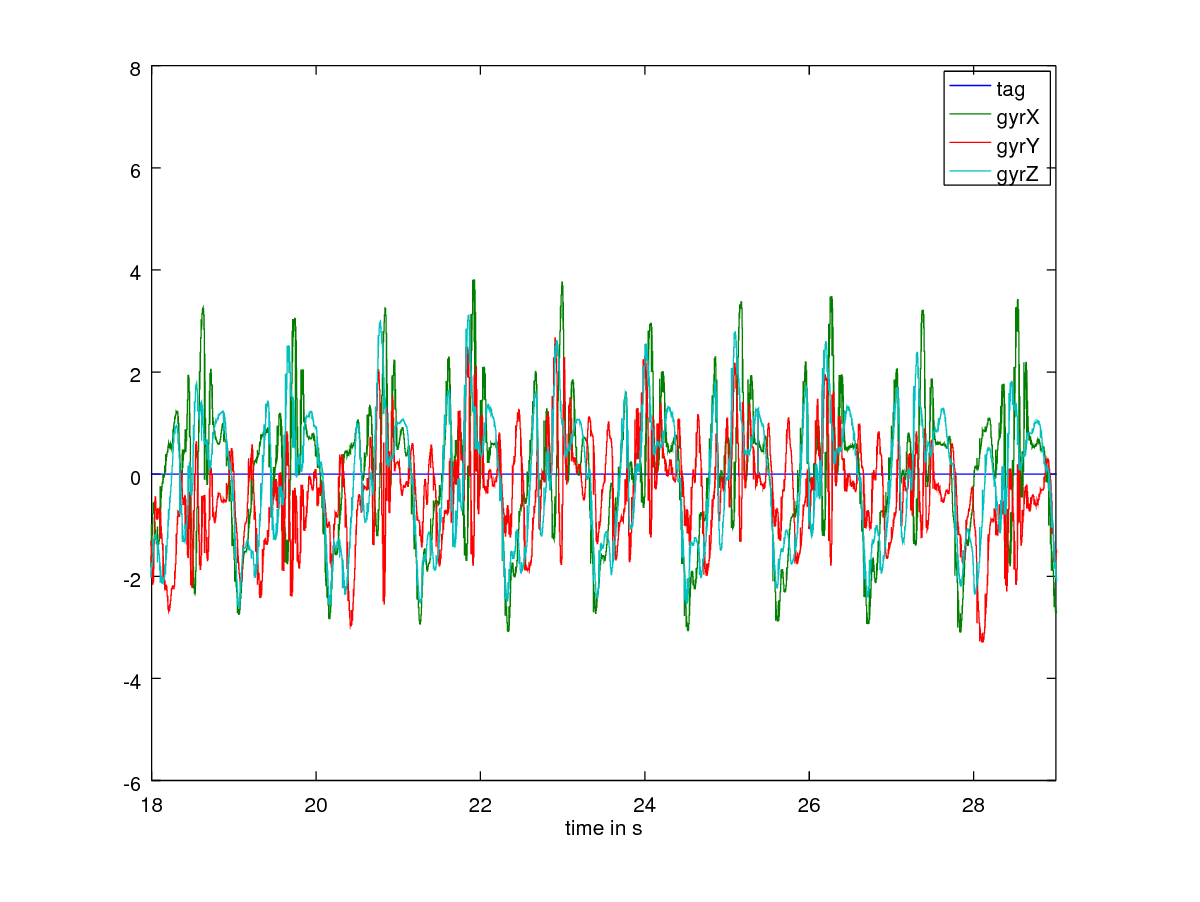
\includegraphics[width=.45\textwidth]{stairsfhdown2_walking_g} &
	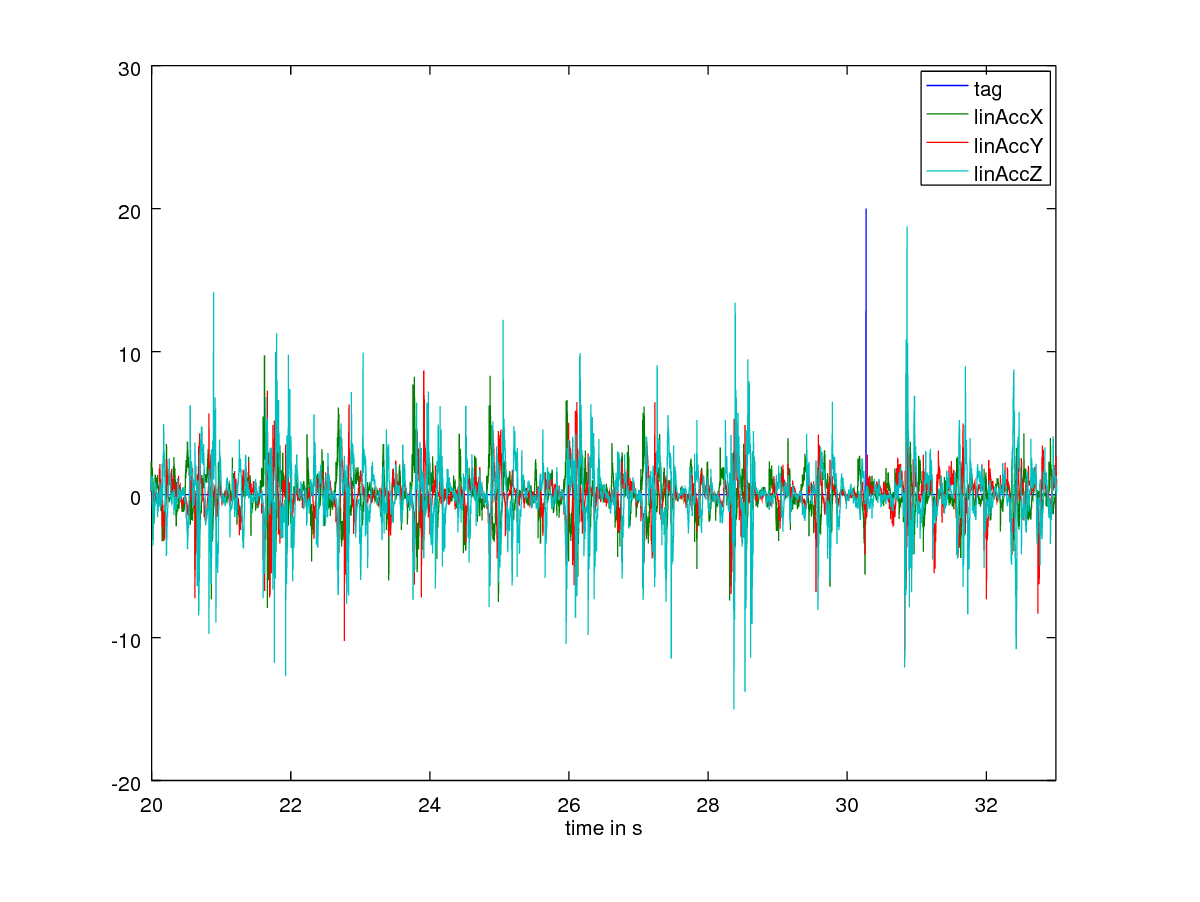
\includegraphics[width=.45\textwidth]{stairsfhdown2_walking_la} 
	\\
	(c) & (d)
	\\[4pt]	%vertical extra spacing (4 points)
	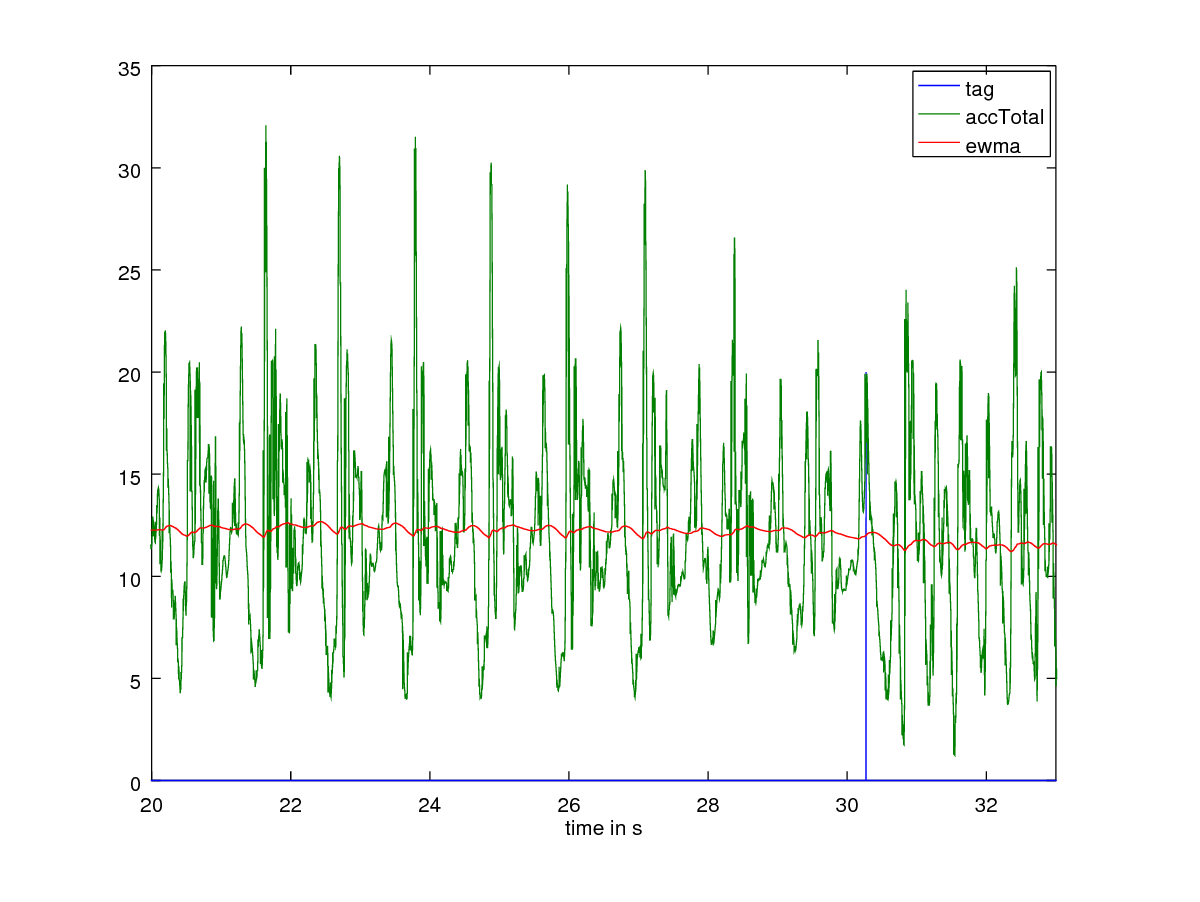
\includegraphics[width=.45\textwidth]{stairsfhdown2_walking_atotal} &
	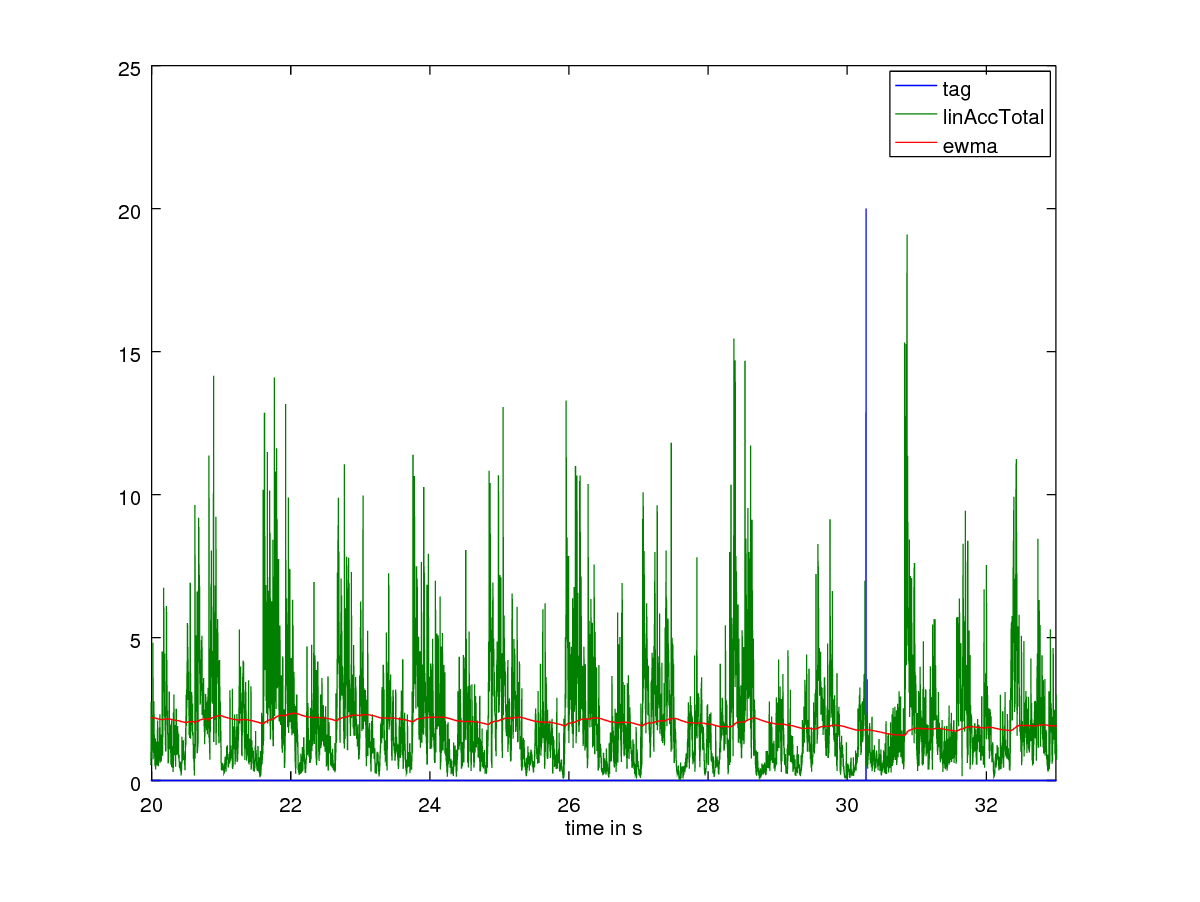
\includegraphics[width=.45\textwidth]{stairsfhdown2_walking_latotal} 
	\\
	(e) & (f)
	\end{tabular}
	%
	\caption{Test case 2}
	\label{fig:Test_case_2_walking}
\end{figure}


%%%----------------------------------------------------------
\section{Test case 3}
%%%----------------------------------------------------------
Test case 3 in Fig.~\ref{fig:Test_case_3_walking}
\begin{figure}
	\centering\small
	\setlength{\tabcolsep}{0mm}	% alle Spaltenränder auf 0mm
	\begin{tabular}{c@{\hspace{12mm}}c} % mittlerer Abstand = 12mm
	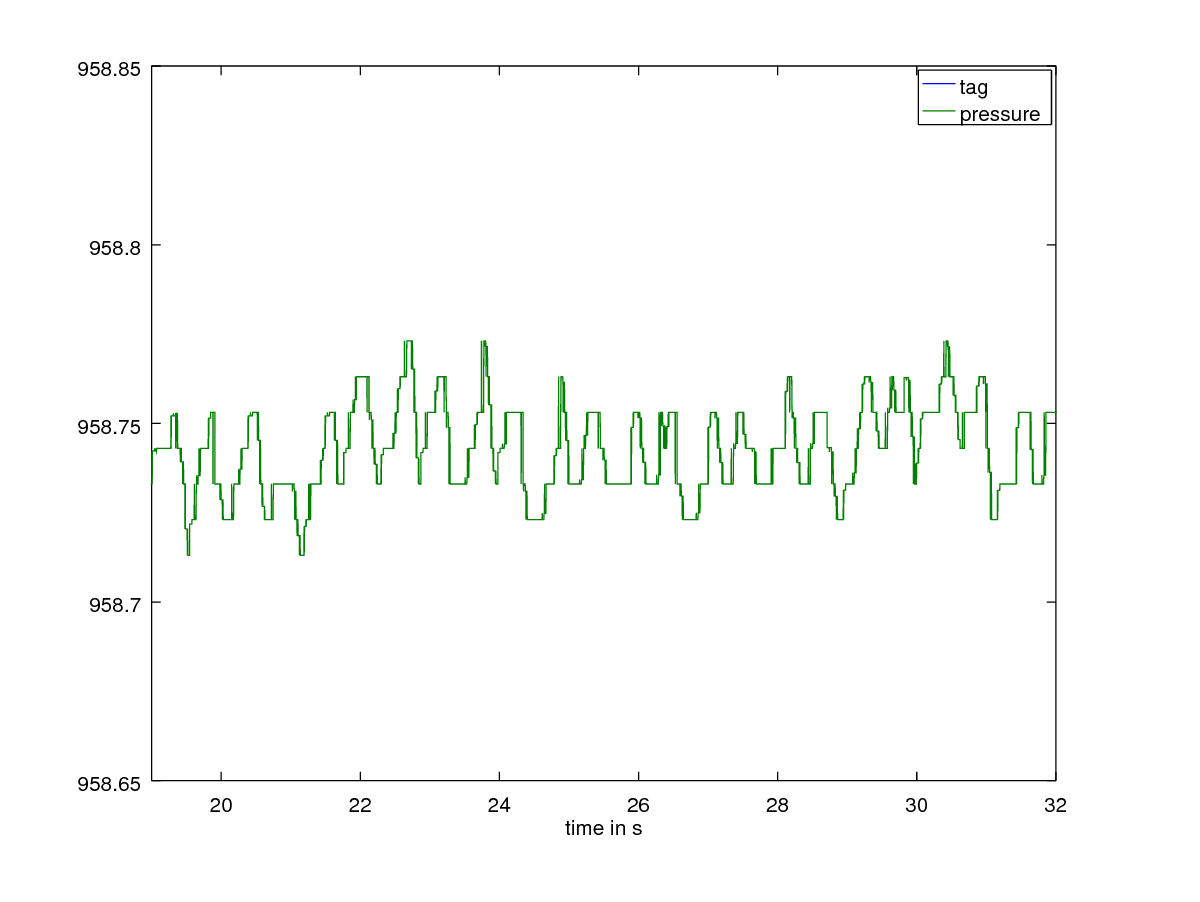
\includegraphics[width=.45\textwidth]{stairsfhdown6_walking_p} &
	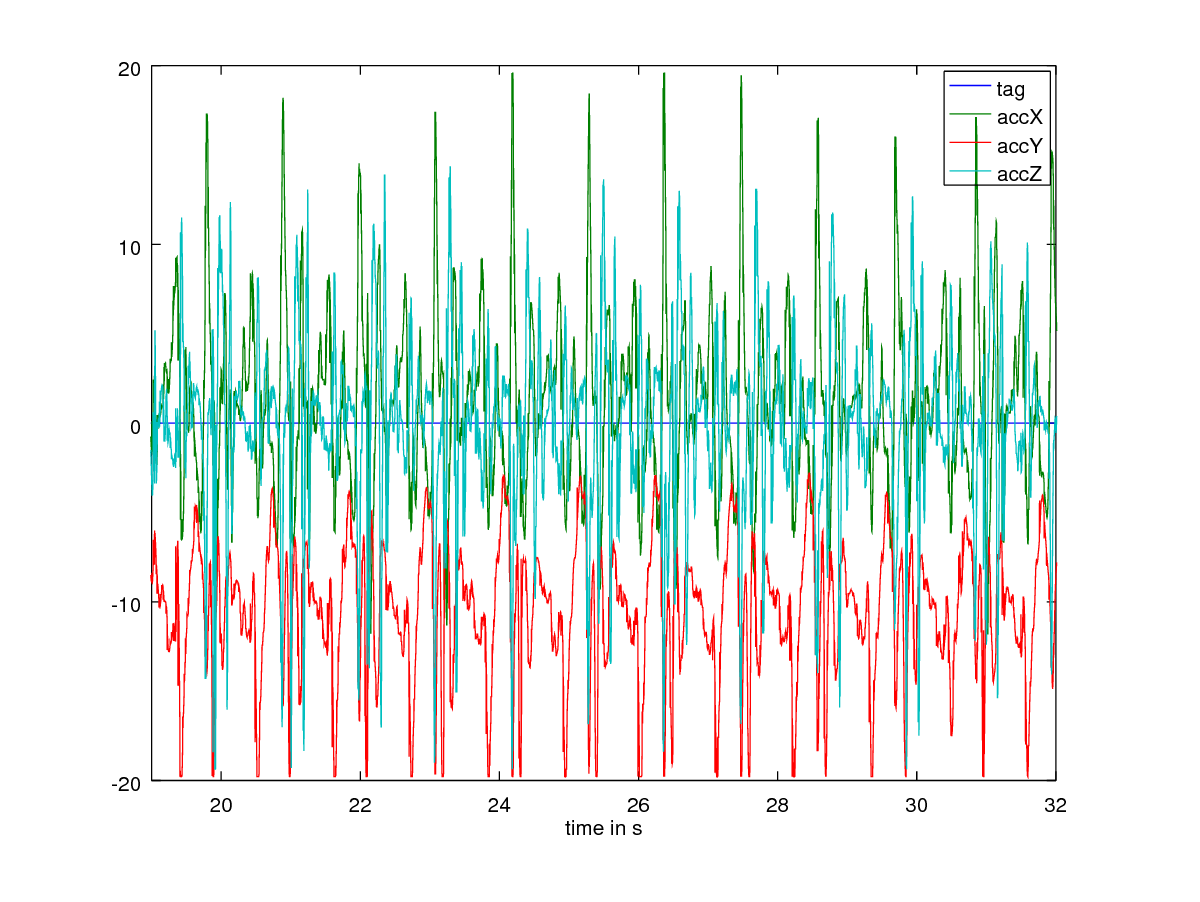
\includegraphics[width=.45\textwidth]{stairsfhdown6_walking_a} 
	\\
	(a) & (b)
	\\[4pt]	%vertical extra spacing (4 points)
	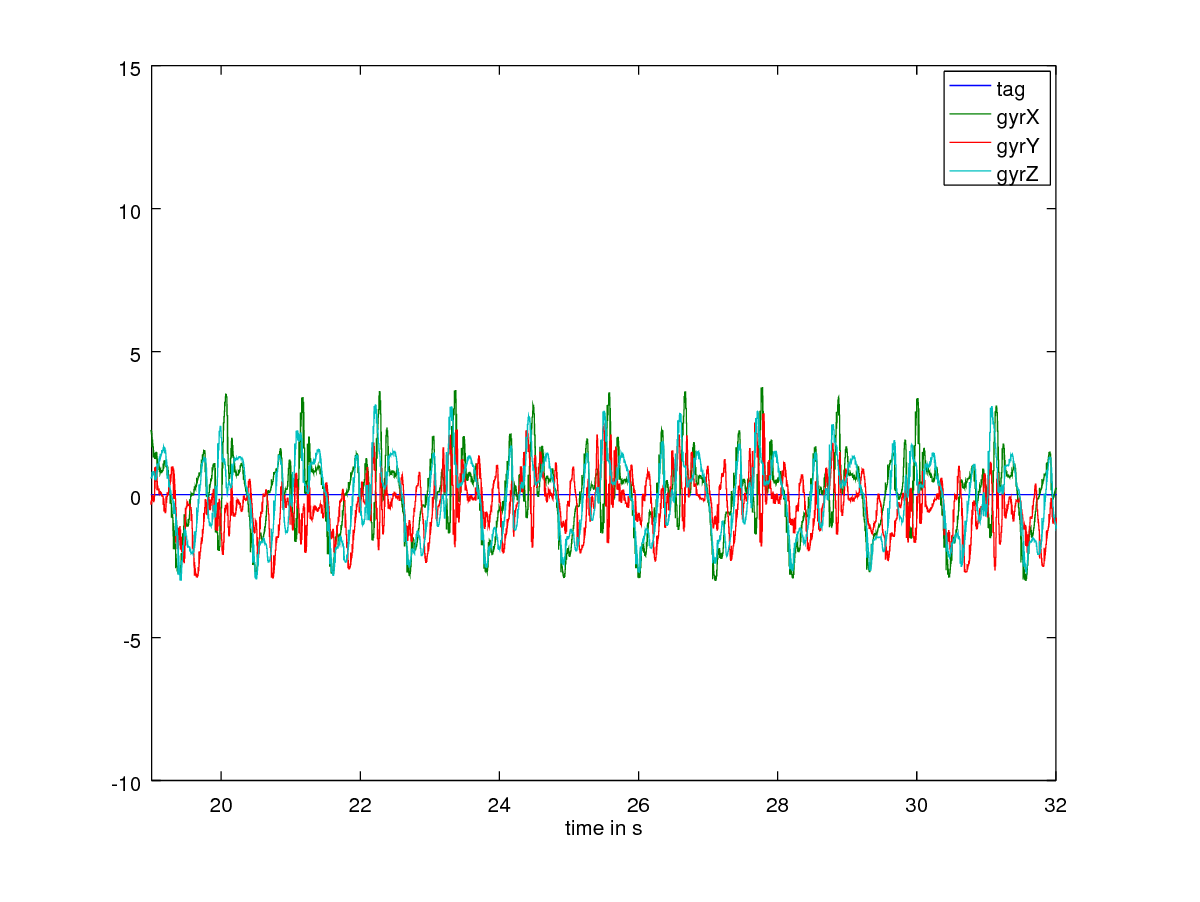
\includegraphics[width=.45\textwidth]{stairsfhdown6_walking_g} &
	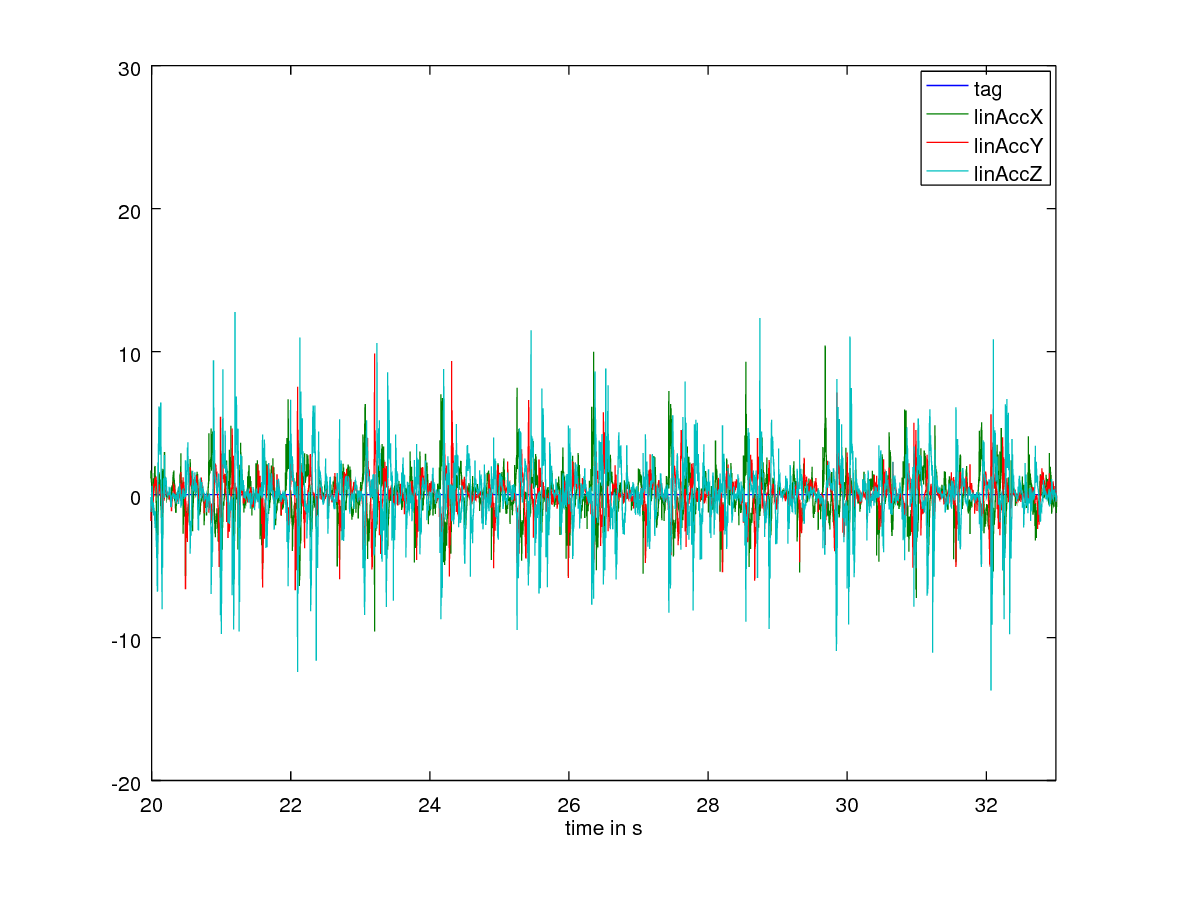
\includegraphics[width=.45\textwidth]{stairsfhdown6_walking_la} 
	\\
	(c) & (d)
	\\[4pt]	%vertical extra spacing (4 points)
	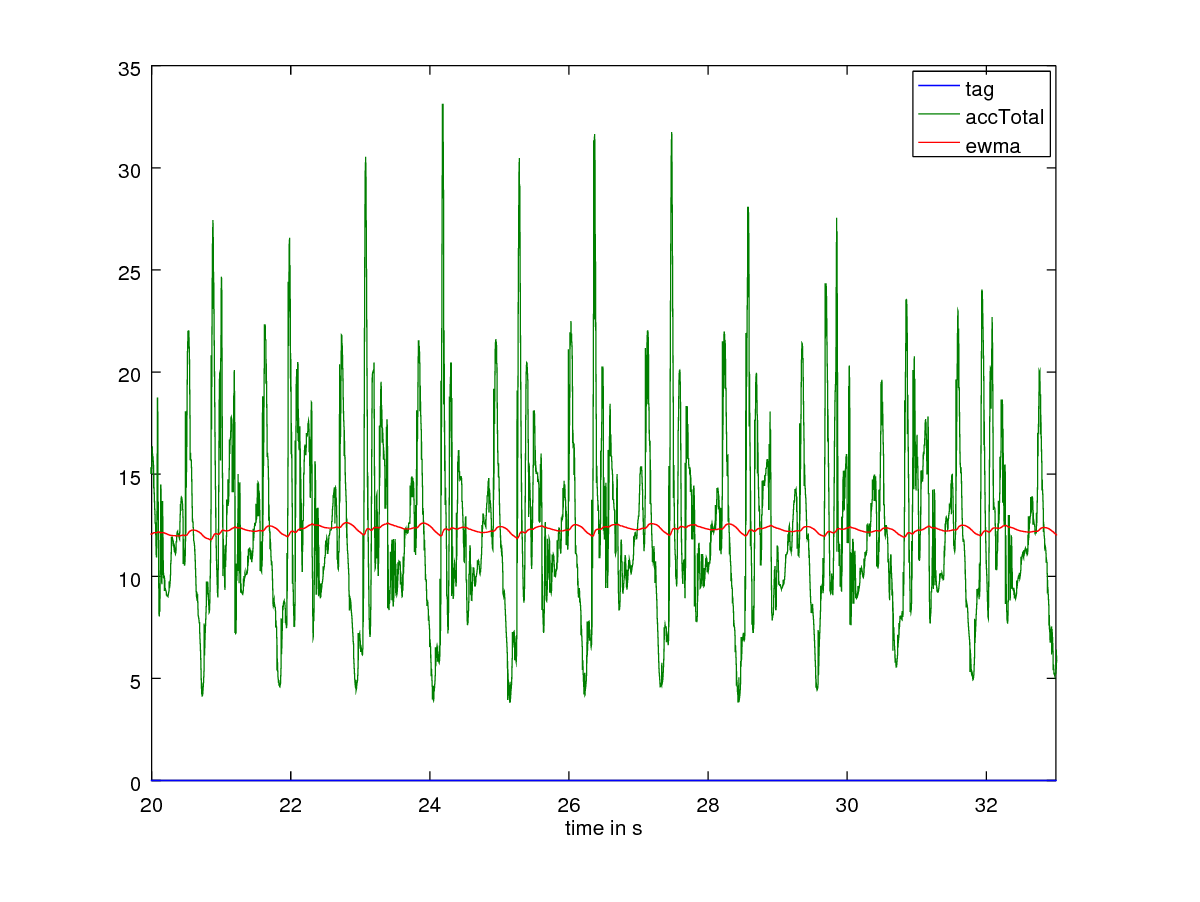
\includegraphics[width=.45\textwidth]{stairsfhdown6_walking_atotal} &
	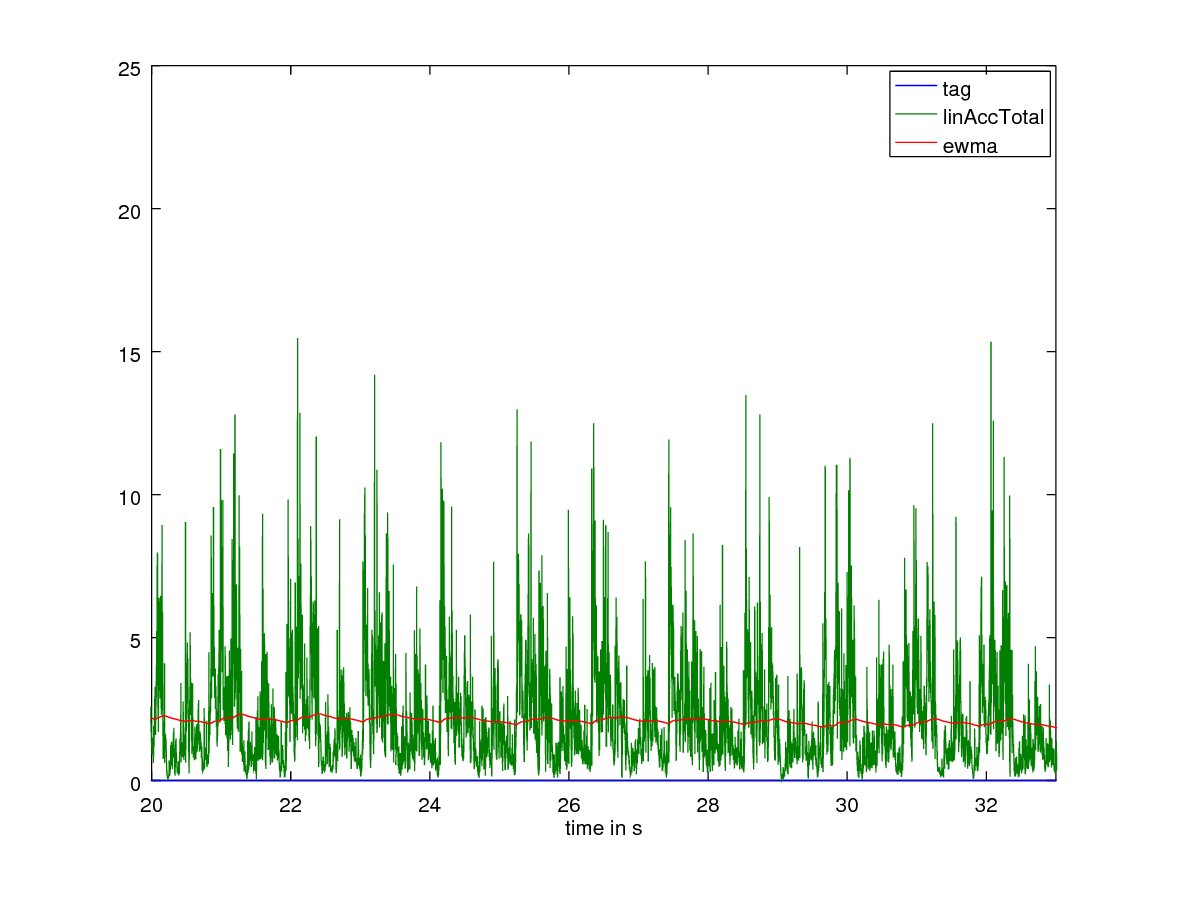
\includegraphics[width=.45\textwidth]{stairsfhdown6_walking_latotal} 
	\\
	(e) & (f)
	\end{tabular}
	%
	\caption{Test case 3}
	\label{fig:Test_case_3_walking}
\end{figure}

%%%----------------------------------------------------------
\section{Test case 4}
%%%----------------------------------------------------------
Test case 4 in Fig.~\ref{fig:Test_case_4_walking}
\begin{figure}
	\centering\small
	\setlength{\tabcolsep}{0mm}	% alle Spaltenränder auf 0mm
	\begin{tabular}{c@{\hspace{12mm}}c} % mittlerer Abstand = 12mm
	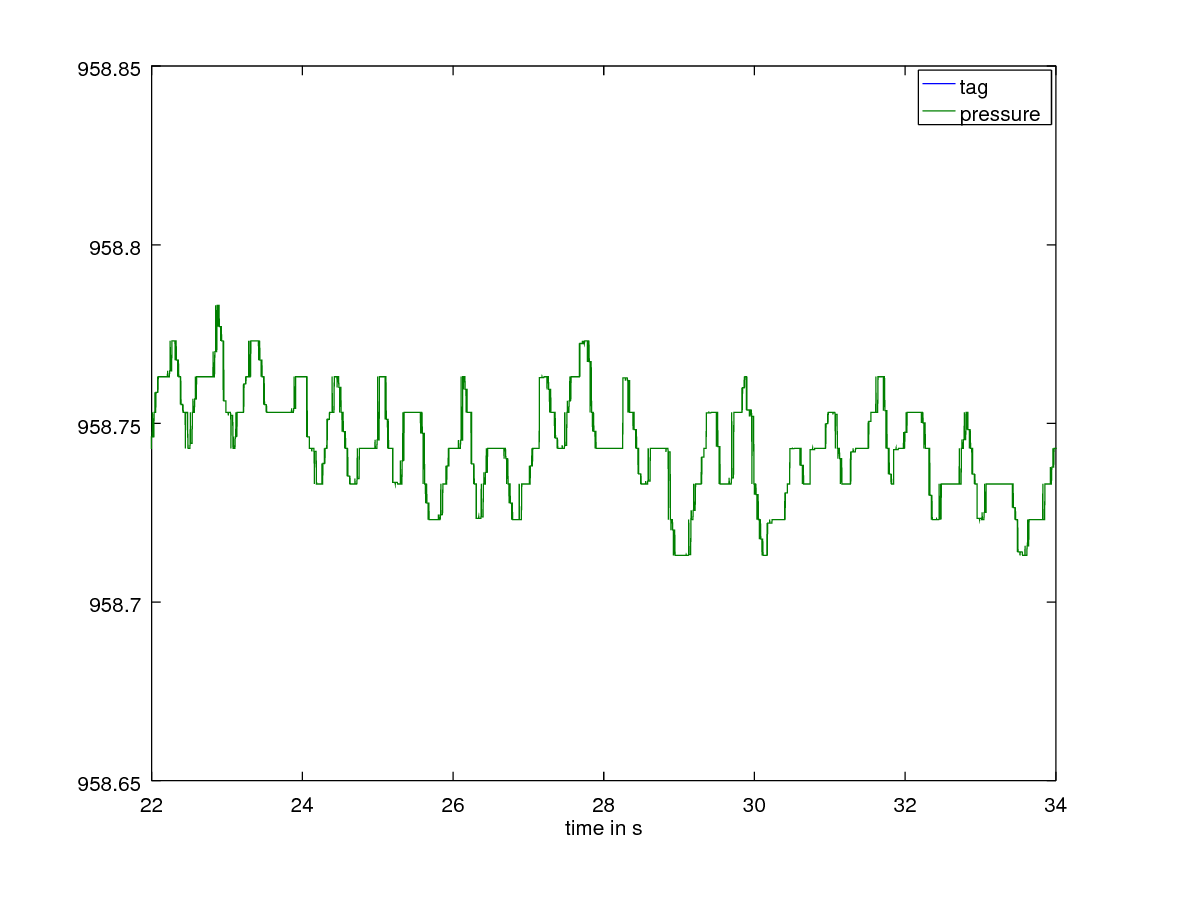
\includegraphics[width=.45\textwidth]{stairsfhdown10_walking_p} &
	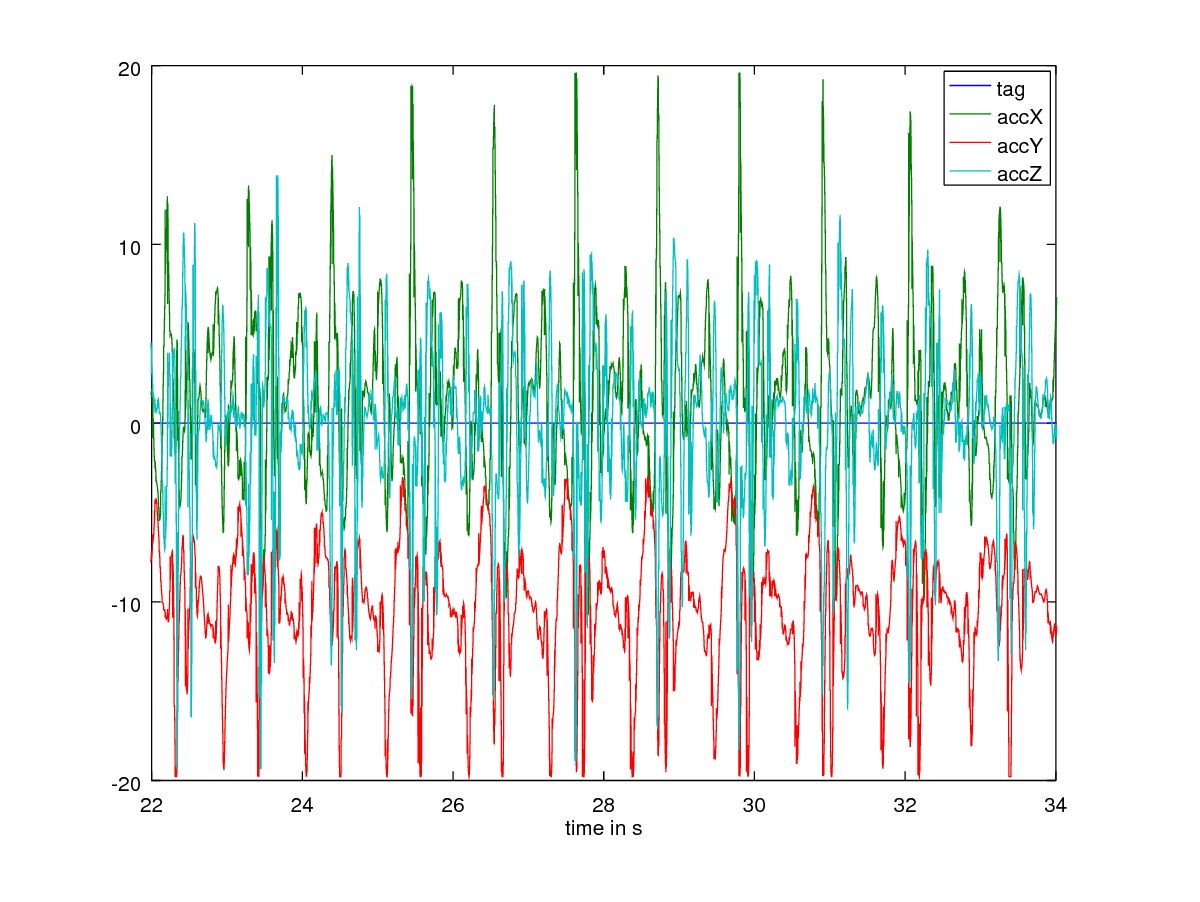
\includegraphics[width=.45\textwidth]{stairsfhdown10_walking_a} 
	\\
	(a) & (b)
	\\[4pt]	%vertical extra spacing (4 points)
	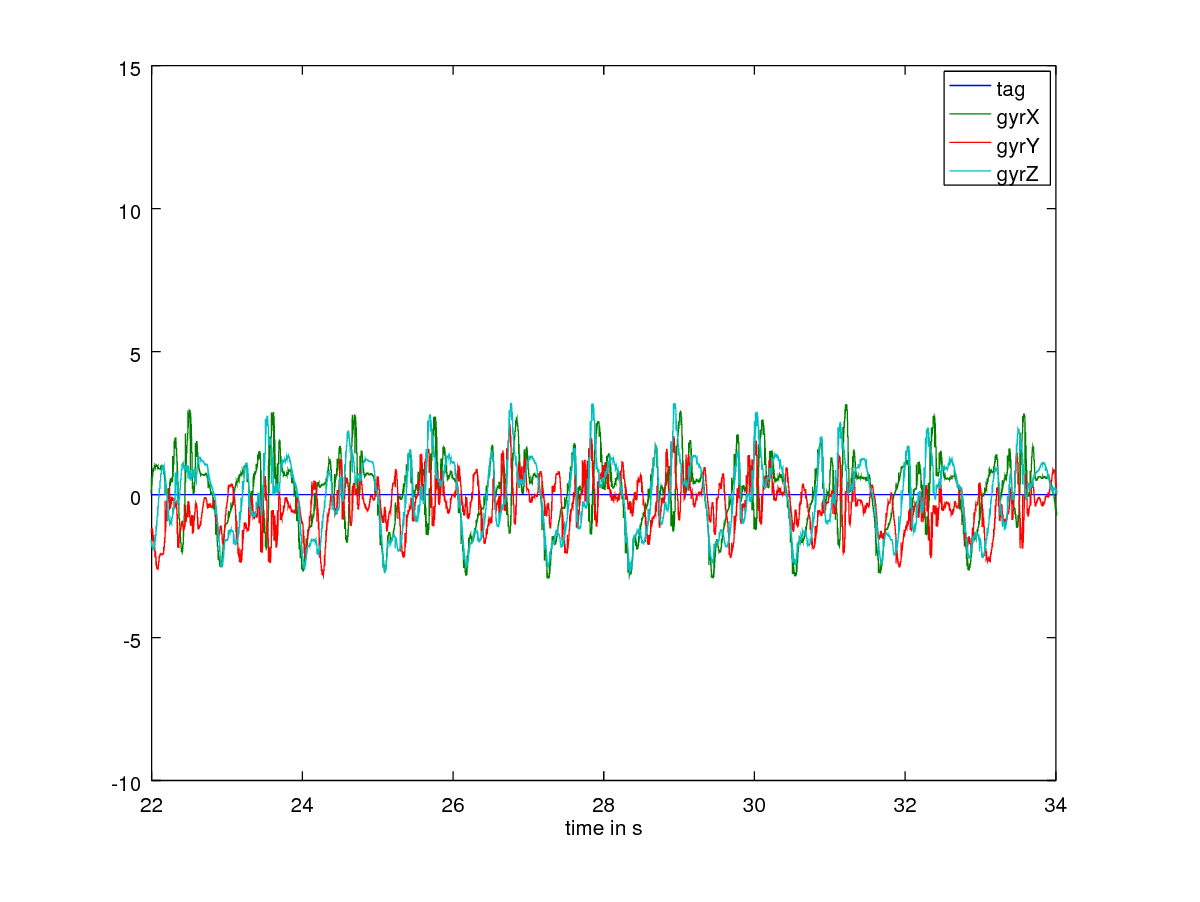
\includegraphics[width=.45\textwidth]{stairsfhdown10_walking_g} &
	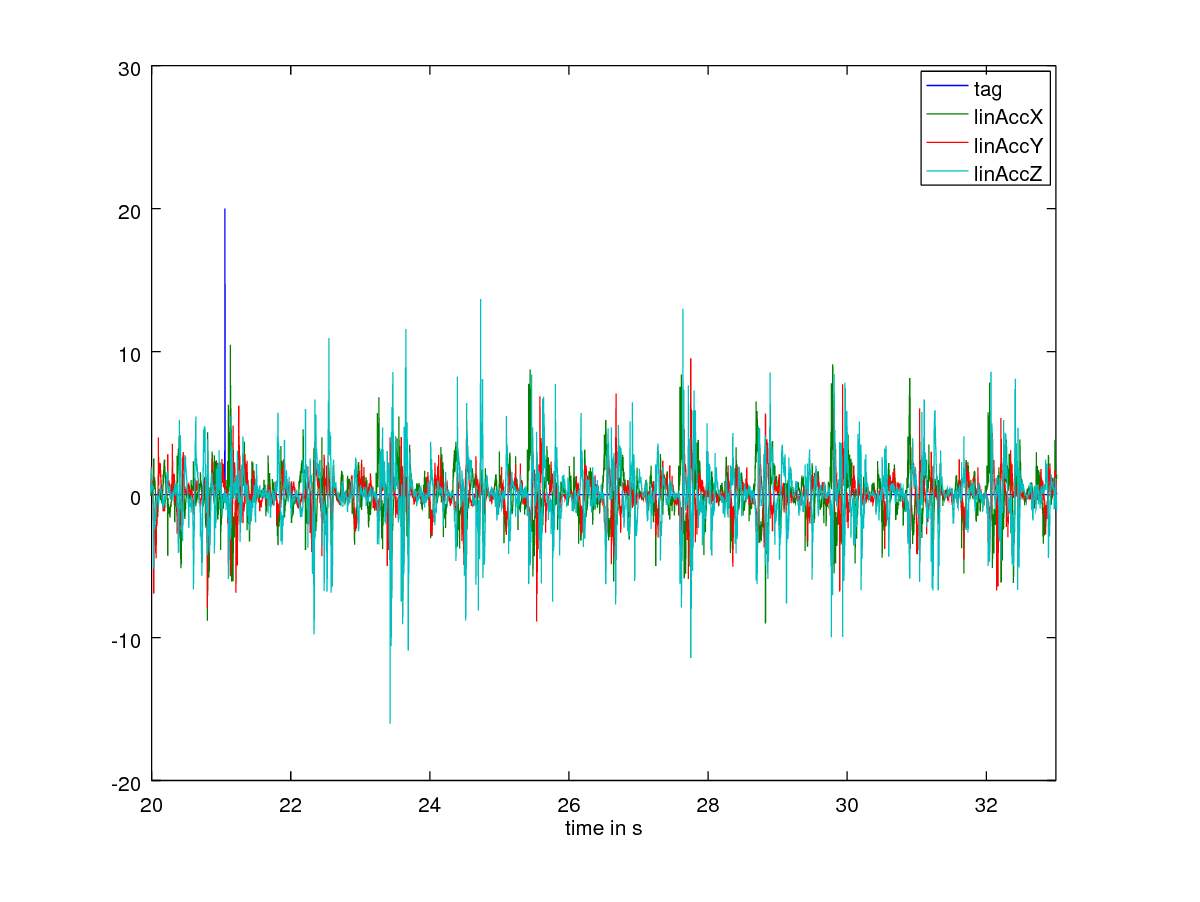
\includegraphics[width=.45\textwidth]{stairsfhdown10_walking_la} 
	\\
	(c) & (d)
	\\[4pt]	%vertical extra spacing (4 points)
	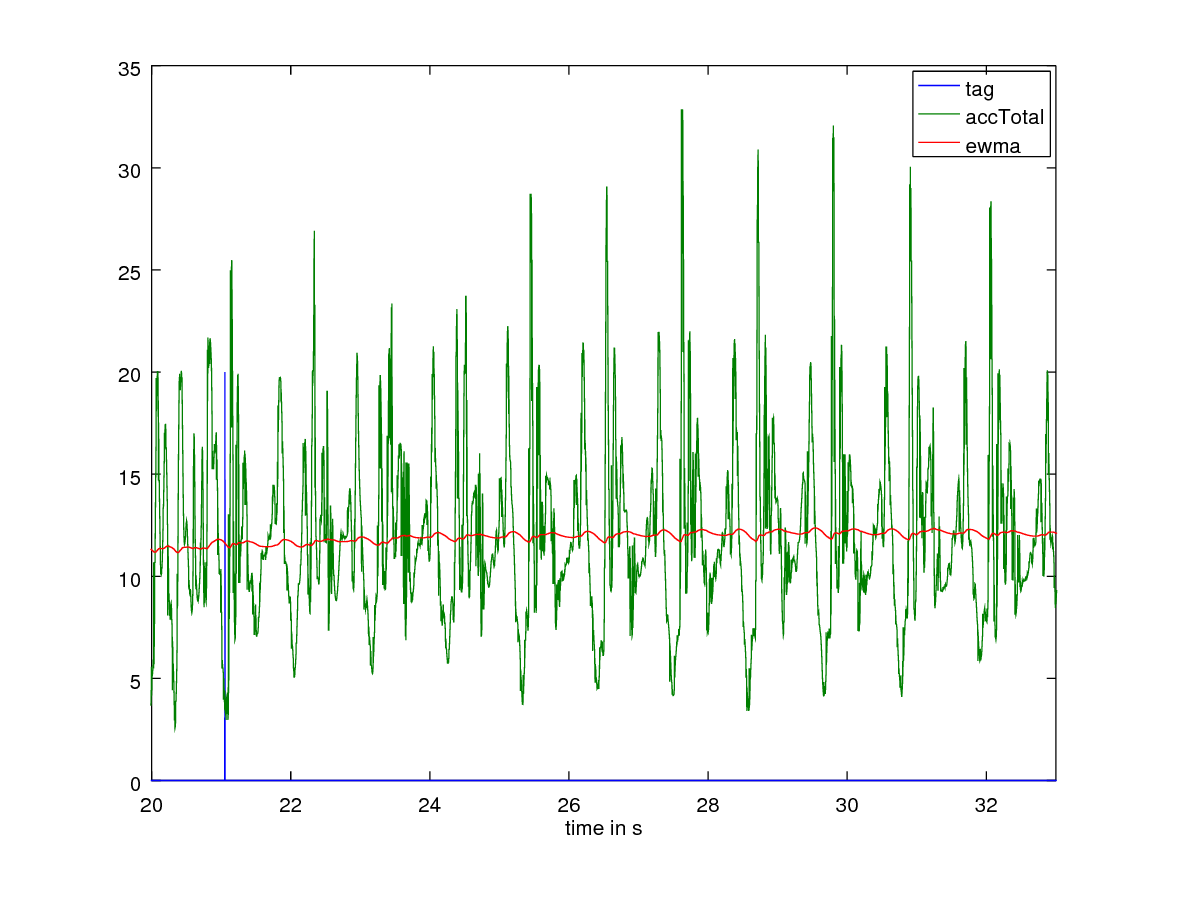
\includegraphics[width=.45\textwidth]{stairsfhdown10_walking_atotal} &
	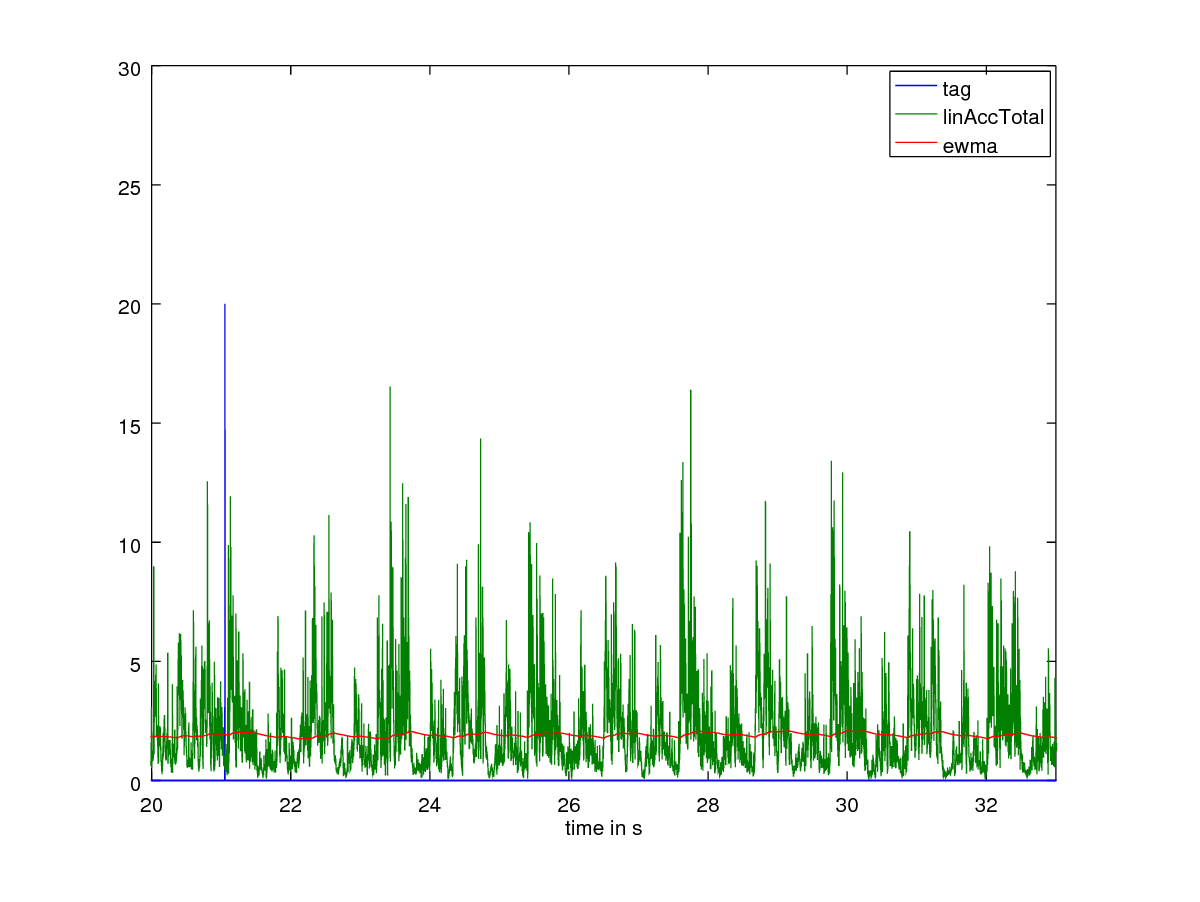
\includegraphics[width=.45\textwidth]{stairsfhdown10_walking_latotal} 
	\\
	(e) & (f)
		\end{tabular}
	%
	\caption{Test case 4}
	\label{fig:Test_case_4_walking}
\end{figure}

%%%----------------------------------------------------------
\section{Test case 5}
%%%----------------------------------------------------------
Test case 5 in Fig.~\ref{fig:Test_case_5_walking}
\begin{figure}
	\centering\small
	\setlength{\tabcolsep}{0mm}	% alle Spaltenränder auf 0mm
	\begin{tabular}{c@{\hspace{12mm}}c} % mittlerer Abstand = 12mm
		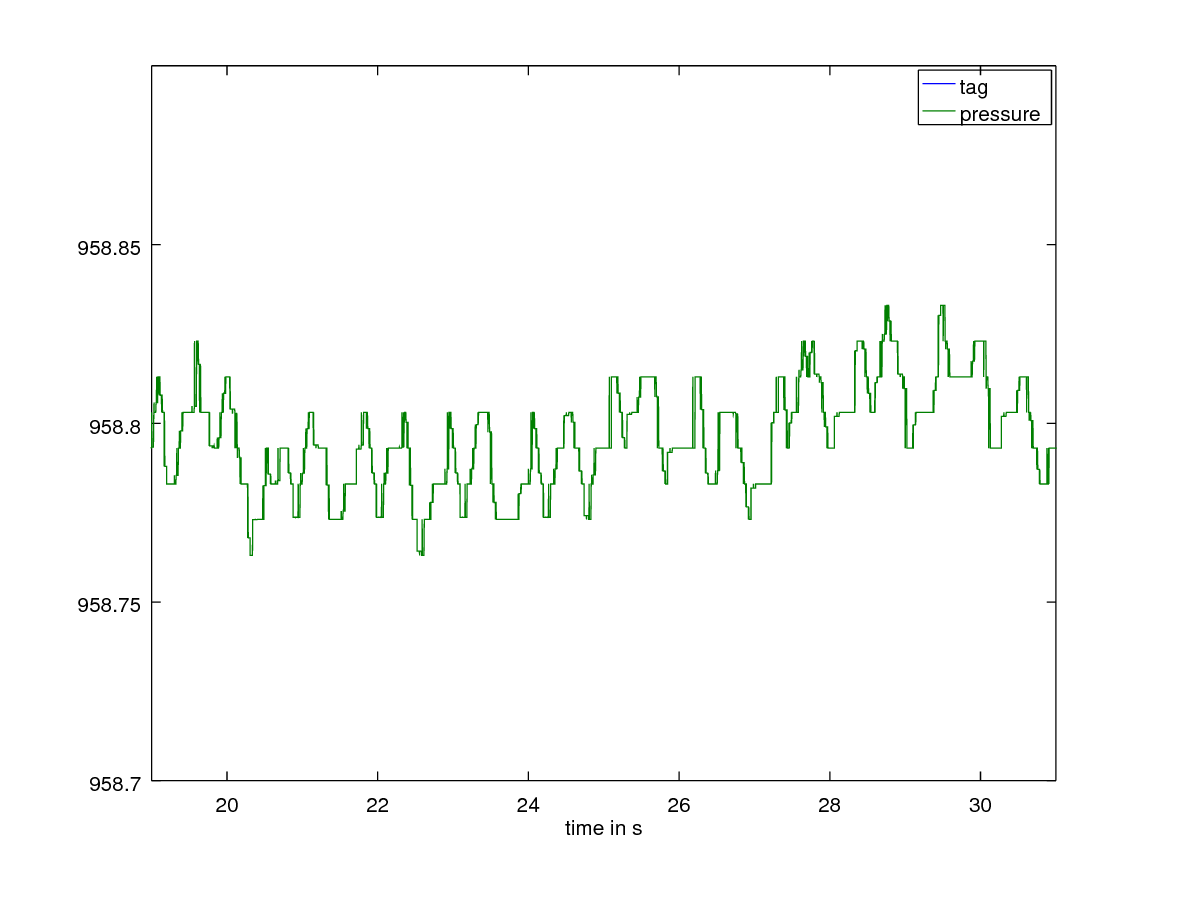
\includegraphics[width=.45\textwidth]{stairsfhdown20_walking_p} &
		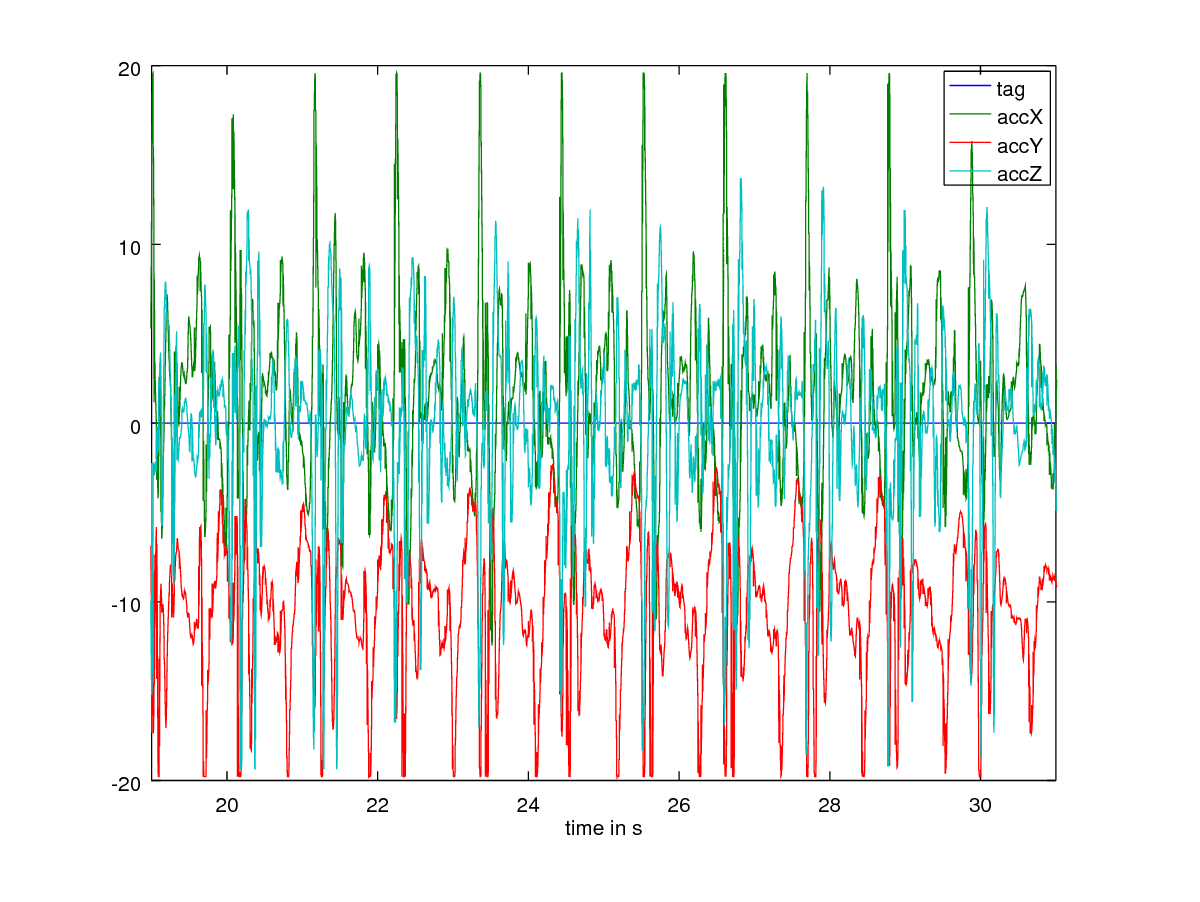
\includegraphics[width=.45\textwidth]{stairsfhdown20_walking_a} 
		\\
		(a) & (b)
		\\[4pt]	%vertical extra spacing (4 points)
		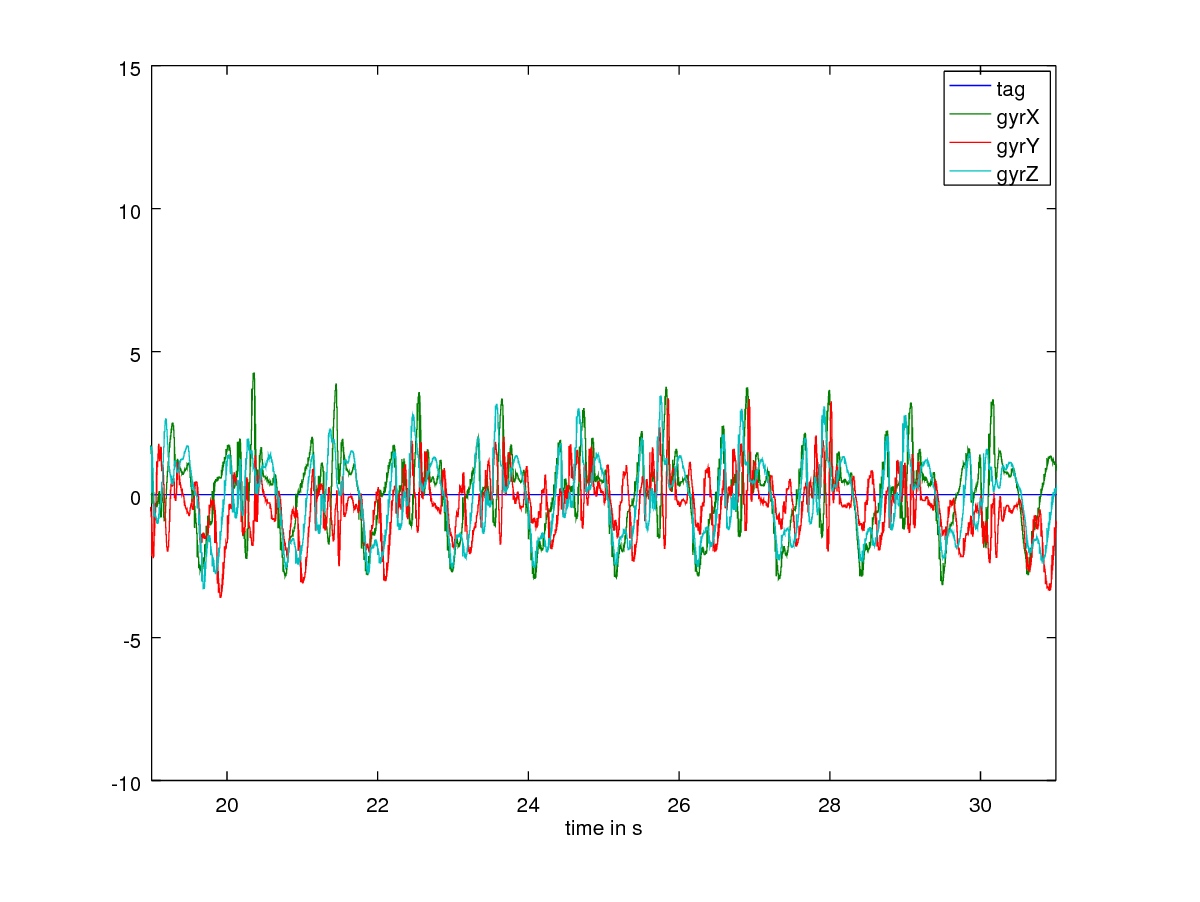
\includegraphics[width=.45\textwidth]{stairsfhdown20_walking_g} &
		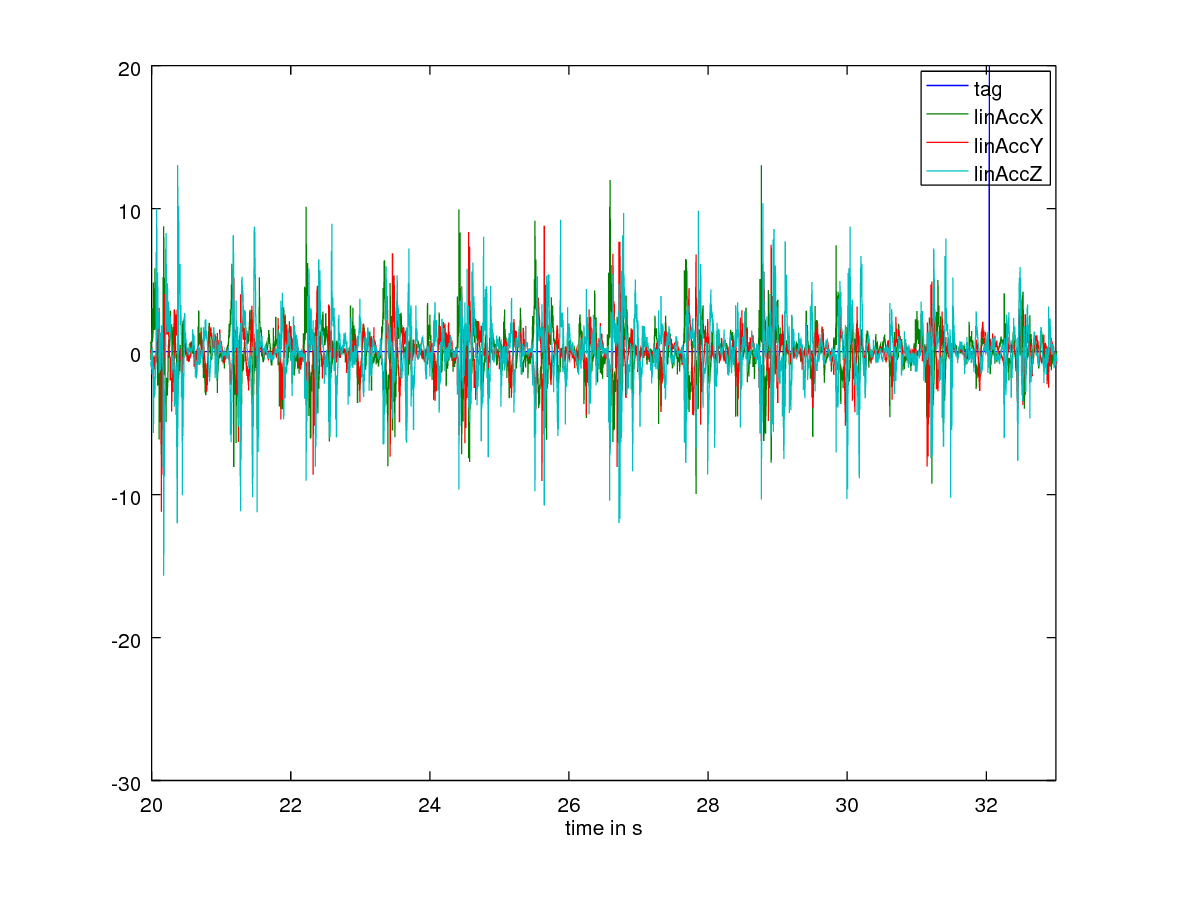
\includegraphics[width=.45\textwidth]{stairsfhdown20_walking_la} 
		\\
		(c) & (d)
		\\[4pt]	%vertical extra spacing (4 points)
		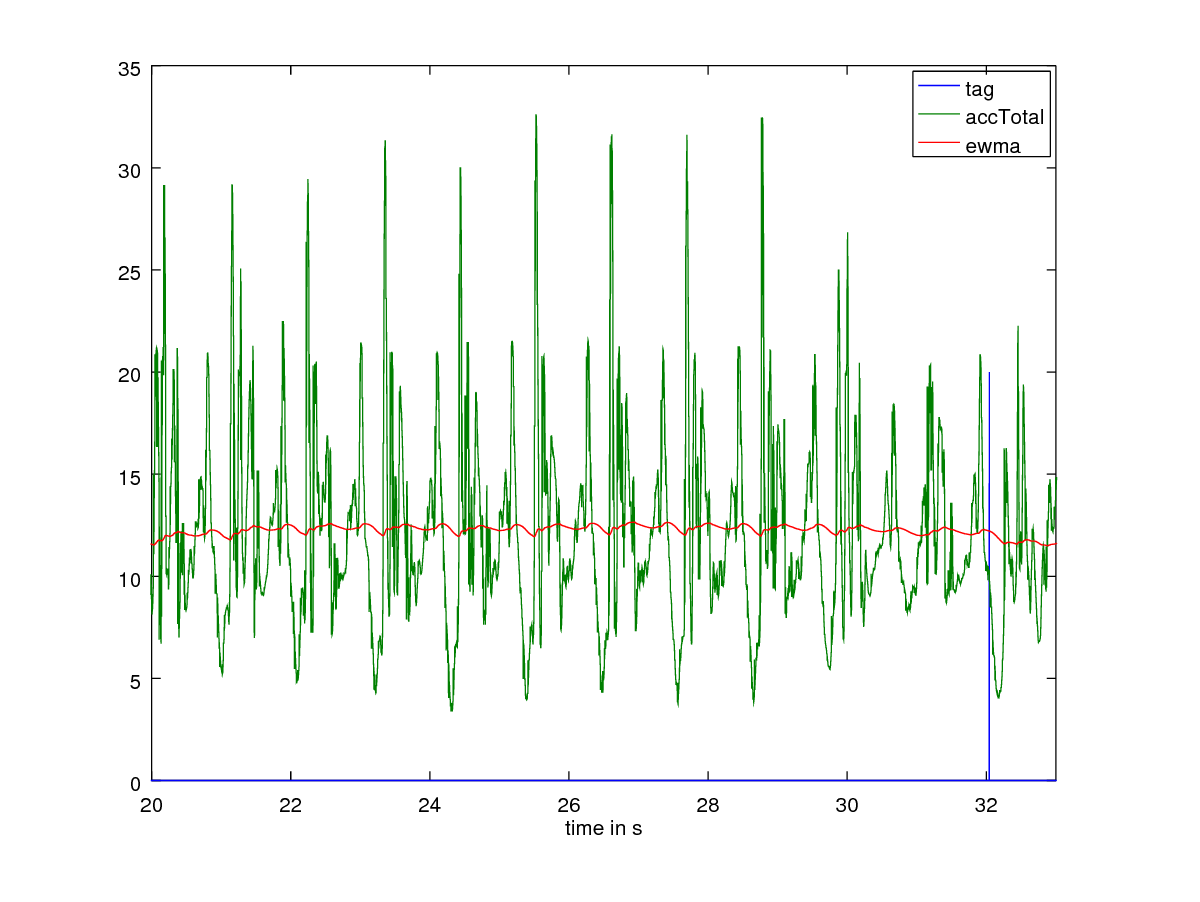
\includegraphics[width=.45\textwidth]{stairsfhdown20_walking_atotal} &
		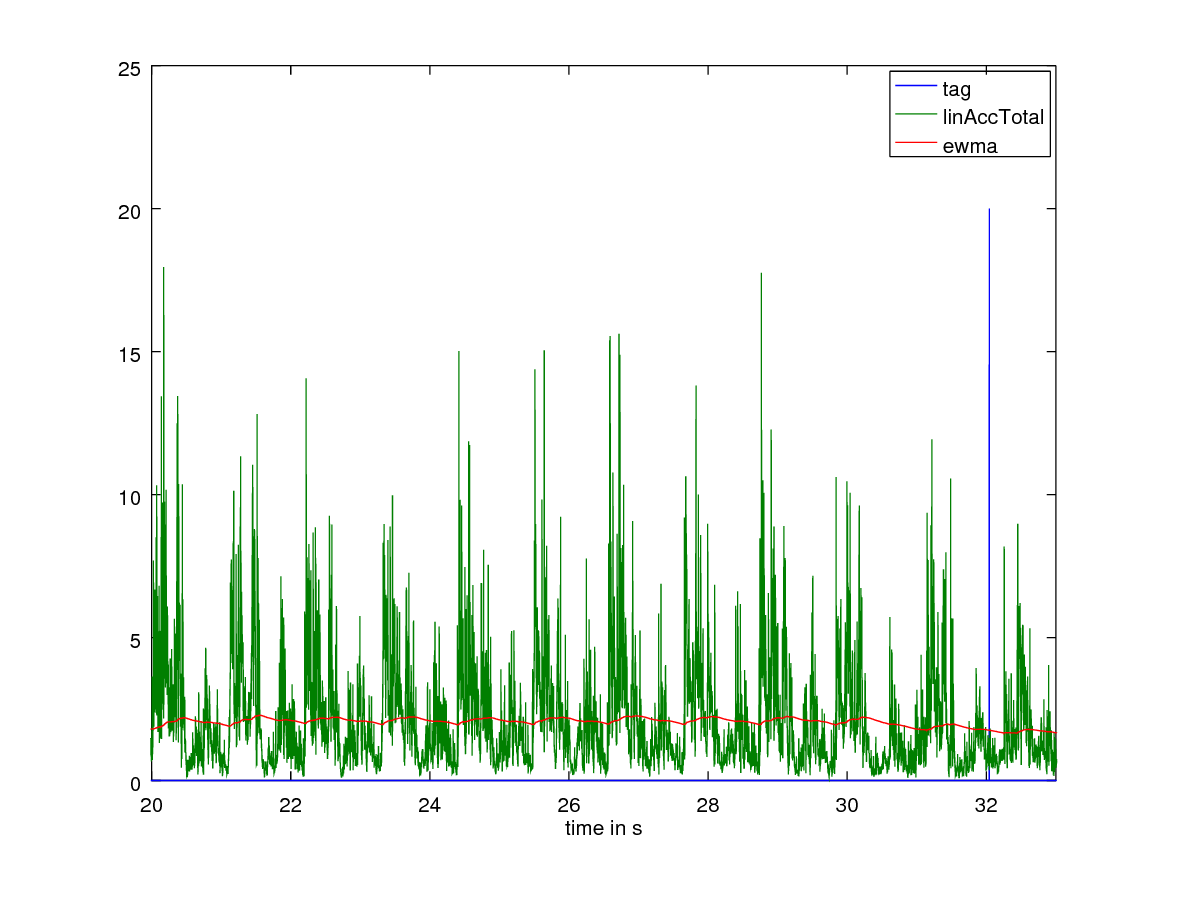
\includegraphics[width=.45\textwidth]{stairsfhdown20_walking_latotal} 
		\\
		(e) & (f)
		\end{tabular}
		%
		\caption{Test case 5}
		\label{fig:Test_case_5_walking}
	\end{figure}
	
%%%----------------------------------------------------------
\section{Test case 6}
%%%----------------------------------------------------------
Test case 6 in Fig.~\ref{fig:Test_case_6_walking}
\begin{figure}
	\centering\small
	\setlength{\tabcolsep}{0mm}	% alle Spaltenränder auf 0mm
	\begin{tabular}{c@{\hspace{12mm}}c} % mittlerer Abstand = 12mm
		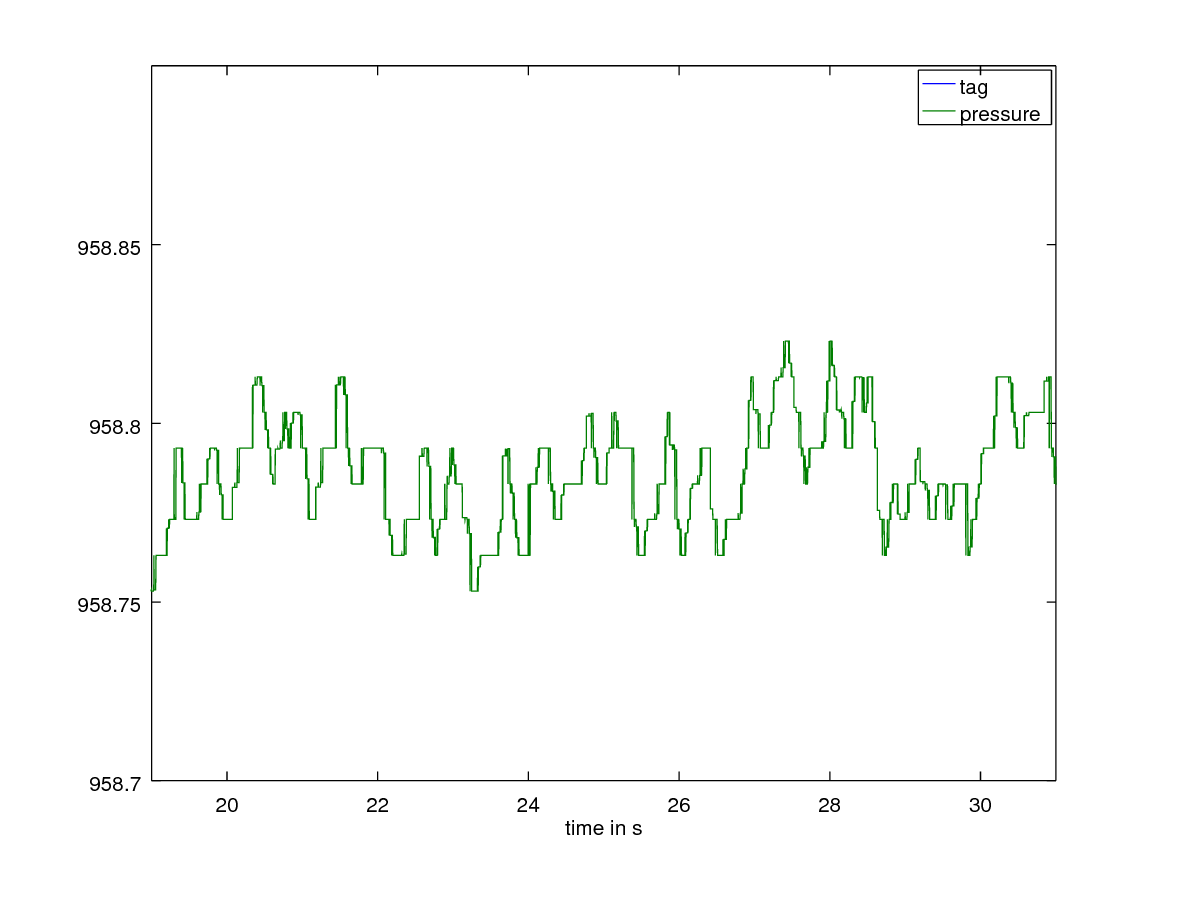
\includegraphics[width=.45\textwidth]{stairsfhdown50_walking_p} &
		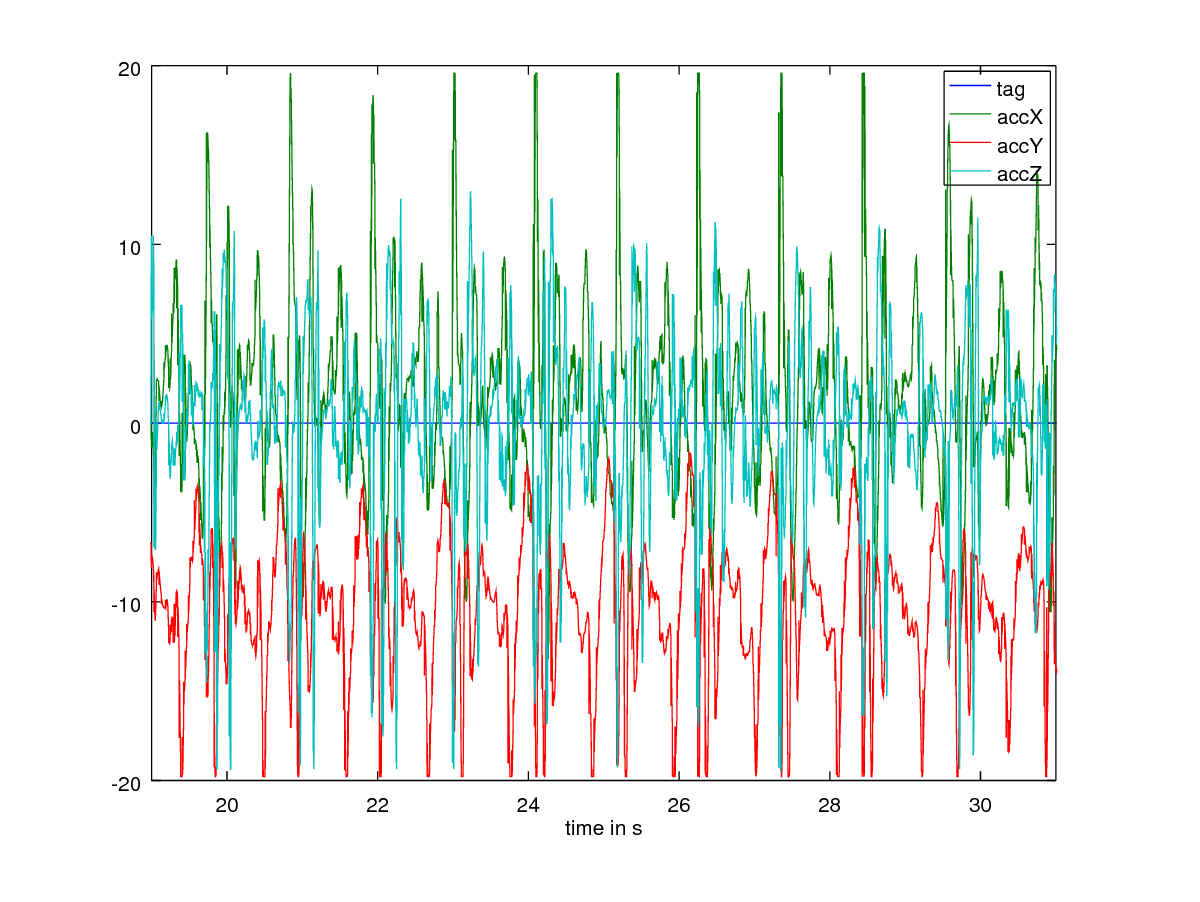
\includegraphics[width=.45\textwidth]{stairsfhdown50_walking_a} 
		\\
		(a) & (b)
		\\[4pt]	%vertical extra spacing (4 points)
		\includegraphics[width=.45\textwidth]{stairsfhdown50_walking_g} &
		\includegraphics[width=.45\textwidth]{stairsfhdown50_walking_la} 
		\\
		(c) & (d)
		\\[4pt]	%vertical extra spacing (4 points)
		\includegraphics[width=.45\textwidth]{stairsfhdown50_walking_atotal} &
		\includegraphics[width=.45\textwidth]{stairsfhdown50_walking_latotal} 
		\\
		(e) & (f)
		\end{tabular}
		%
		\caption{Test case 6}
		\label{fig:Test_case_6_walking}
	\end{figure}
	
	
%%%----------------------------------------------------------
\section{Test case 7}
%%%----------------------------------------------------------
Test case 7 in Fig.~\ref{fig:Test_case_7_walking}
\begin{figure}
	\centering\small
	\setlength{\tabcolsep}{0mm}	% alle Spaltenränder auf 0mm
	\begin{tabular}{c@{\hspace{12mm}}c} % mittlerer Abstand = 12mm
		\includegraphics[width=.45\textwidth]{stairsfhdown70_walking_p} &
		\includegraphics[width=.45\textwidth]{stairsfhdown70_walking_a} 
		\\
		(a) & (b)
		\\[4pt]	%vertical extra spacing (4 points)
		\includegraphics[width=.45\textwidth]{stairsfhdown70_walking_g} &
		\includegraphics[width=.45\textwidth]{stairsfhdown70_walking_la} 
		\\
		(c) & (d)
		\\[4pt]	%vertical extra spacing (4 points)
		\includegraphics[width=.45\textwidth]{stairsfhdown70_walking_atotal} &
		\includegraphics[width=.45\textwidth]{stairsfhdown70_walking_latotal} 
		\\
		(e) & (f)
		\end{tabular}
		%
		\caption{Test case 7}
		\label{fig:Test_case_7_walking}
	\end{figure}
	
	
%%%----------------------------------------------------------
\section{Test case 8}
%%%----------------------------------------------------------
Test case 8 in Fig.~\ref{fig:Test_case_8_walking}
\begin{figure}
	\centering\small
	\setlength{\tabcolsep}{0mm}	% alle Spaltenränder auf 0mm
	\begin{tabular}{c@{\hspace{12mm}}c} % mittlerer Abstand = 12mm
		\includegraphics[width=.45\textwidth]{stairsfhdown100_walking_p} &
		\includegraphics[width=.45\textwidth]{stairsfhdown100_walking_a} 
		\\
		(a) & (b)
		\\[4pt]	%vertical extra spacing (4 points)
		\includegraphics[width=.45\textwidth]{stairsfhdown100_walking_g} &
		\includegraphics[width=.45\textwidth]{stairsfhdown100_walking_la} 
		\\
		(c) & (d)
		\\[4pt]	%vertical extra spacing (4 points)
		\includegraphics[width=.45\textwidth]{stairsfhdown100_walking_atotal} &
		\includegraphics[width=.45\textwidth]{stairsfhdown100_walking_latotal} 
		\\
		(e) & (f)
		\end{tabular}
		%
		\caption{Test case 8}
		\label{fig:Test_case_8_walking}
	\end{figure}
	
%%%----------------------------------------------------------
\section{Test case 9}
%%%----------------------------------------------------------
Test case 9 in Fig.~\ref{fig:Test_case_9_walking}
\begin{figure}
	\centering\small
	\setlength{\tabcolsep}{0mm}	% alle Spaltenränder auf 0mm
	\begin{tabular}{c@{\hspace{12mm}}c} % mittlerer Abstand = 12mm
		\includegraphics[width=.45\textwidth]{stairsfhdowna2_walking_p} &
		\includegraphics[width=.45\textwidth]{stairsfhdowna2_walking_a} 
		\\
		(a) & (b)
		\\[4pt]	%vertical extra spacing (4 points)
		\includegraphics[width=.45\textwidth]{stairsfhdowna2_walking_g} &
		\includegraphics[width=.45\textwidth]{stairsfhdowna2_walking_la} 
		\\
		(c) & (d)
		\\[4pt]	%vertical extra spacing (4 points)
		\includegraphics[width=.45\textwidth]{stairsfhdowna2_walking_atotal} &
		\includegraphics[width=.45\textwidth]{stairsfhdowna2_walking_latotal} 
		\\
		(e) & (f)
		\end{tabular}
		%
		\caption{Test case 9}
		\label{fig:Test_case_9_walking}
	\end{figure}
	
%%%----------------------------------------------------------
\section{Test case 10}
%%%----------------------------------------------------------
Test case 10 in Fig.~\ref{fig:Test_case_10_walking}
\begin{figure}
	\centering\small
	\setlength{\tabcolsep}{0mm}	% alle Spaltenränder auf 0mm
	\begin{tabular}{c@{\hspace{12mm}}c} % mittlerer Abstand = 12mm
		\includegraphics[width=.45\textwidth]{stairsfhdownf1_walking_p} &
		\includegraphics[width=.45\textwidth]{stairsfhdownf1_walking_a} 
		\\
		(a) & (b)
		\\[4pt]	%vertical extra spacing (4 points)
		\includegraphics[width=.45\textwidth]{stairsfhdownf1_walking_g} &
		\includegraphics[width=.45\textwidth]{stairsfhdownf1_walking_la} 
		\\
		(c) & (d)
		\\[4pt]	%vertical extra spacing (4 points)
		\includegraphics[width=.45\textwidth]{stairsfhdownf1_walking_atotal} &
		\includegraphics[width=.45\textwidth]{stairsfhdownf1_walking_latotal} 
		\\
		(e) & (f)
		\end{tabular}
		%
		\caption{Test case 10}
		\label{fig:Test_case_10_walking}
	\end{figure}

%%%----------------------------------------------------------
%%%----------------------------------------------------------
%%%----------------------------------------------------------
%%%----------------------------------------------------------
%%%----------------------------------------------------------
\chapter{Stairs}
%%%----------------------------------------------------------

The activity "stairs" will be analyzed here with graphics.
%%%----------------------------------------------------------
\section{Test case 1}
%%%----------------------------------------------------------
Test case 1 in Fig.~\ref{fig:Test_case_stairs_1}
\begin{figure}
	\centering\small
	\setlength{\tabcolsep}{0mm}	% alle Spaltenränder auf 0mm
	\begin{tabular}{c@{\hspace{12mm}}c} % mittlerer Abstand = 12mm
		\includegraphics[width=.45\textwidth]{stairsfhdown_p} &
		\includegraphics[width=.45\textwidth]{stairsfhdown_a} 
		\\
		(a) & (b)
		\\[4pt]	%vertical extra spacing (4 points)
		\includegraphics[width=.45\textwidth]{stairsfhdown_g} &
		\includegraphics[width=.45\textwidth]{stairsfhdown_la} 
		\\
		(c) & (d)
		\\[4pt]	%vertical extra spacing (4 points)
		\includegraphics[width=.45\textwidth]{stairsfhdown_atotal} &
		\includegraphics[width=.45\textwidth]{stairsfhdown_latotal} 
		\\
		(e) & (f)
	\end{tabular}
	%
	\caption{Test case 1}
	\label{fig:Test_case_stairs_1}
\end{figure}

%%%----------------------------------------------------------
\section{Test case 2}
%%%----------------------------------------------------------

Test case 2 in Fig.~\ref{fig:Test_case_stairs_2}
\begin{figure}
	\centering\small
	\setlength{\tabcolsep}{0mm}	% alle Spaltenränder auf 0mm
	\begin{tabular}{c@{\hspace{12mm}}c} % mittlerer Abstand = 12mm
		\includegraphics[width=.45\textwidth]{stairsfhdown2_p} &
		\includegraphics[width=.45\textwidth]{stairsfhdown2_a} 
		\\
		(a) & (b)
		\\[4pt]	%vertical extra spacing (4 points)
		\includegraphics[width=.45\textwidth]{stairsfhdown2_g} &
		\includegraphics[width=.45\textwidth]{stairsfhdown2_la} 
		\\
		(c) & (d)
		\\[4pt]	%vertical extra spacing (4 points)
		\includegraphics[width=.45\textwidth]{stairsfhdown2_atotal} &
		\includegraphics[width=.45\textwidth]{stairsfhdown2_latotal} 
		\\
		(e) & (f)
	\end{tabular}
	%
	\caption{Test case 2}
	\label{fig:Test_case_stairs_2}
\end{figure}


%%%----------------------------------------------------------
\section{Test case 3}
%%%----------------------------------------------------------
Test case 3 in Fig.~\ref{fig:Test_case_stairs_3}
\begin{figure}
	\centering\small
	\setlength{\tabcolsep}{0mm}	% alle Spaltenränder auf 0mm
	\begin{tabular}{c@{\hspace{12mm}}c} % mittlerer Abstand = 12mm
		\includegraphics[width=.45\textwidth]{stairsfhdown6_p} &
		\includegraphics[width=.45\textwidth]{stairsfhdown6_a} 
		\\
		(a) & (b)
		\\[4pt]	%vertical extra spacing (4 points)
		\includegraphics[width=.45\textwidth]{stairsfhdown6_g} &
		\includegraphics[width=.45\textwidth]{stairsfhdown6_la} 
		\\
		(c) & (d)
		\\[4pt]	%vertical extra spacing (4 points)
		\includegraphics[width=.45\textwidth]{stairsfhdown6_atotal} &
		\includegraphics[width=.45\textwidth]{stairsfhdown6_latotal} 
		\\
		(e) & (f)
	\end{tabular}
	%
	\caption{Test case 3}
	\label{fig:Test_case_stairs_3}
\end{figure}

%%%----------------------------------------------------------
\section{Test case 4}
%%%----------------------------------------------------------
Test case 4 in Fig.~\ref{fig:Test_case_stairs_4}
\begin{figure}
	\centering\small
	\setlength{\tabcolsep}{0mm}	% alle Spaltenränder auf 0mm
	\begin{tabular}{c@{\hspace{12mm}}c} % mittlerer Abstand = 12mm
		\includegraphics[width=.45\textwidth]{stairsfhdown10_p} &
		\includegraphics[width=.45\textwidth]{stairsfhdown10_a} 
		\\
		(a) & (b)
		\\[4pt]	%vertical extra spacing (4 points)
		\includegraphics[width=.45\textwidth]{stairsfhdown10_g} &
		\includegraphics[width=.45\textwidth]{stairsfhdown10_la} 
		\\
		(c) & (d)
		\\[4pt]	%vertical extra spacing (4 points)
		\includegraphics[width=.45\textwidth]{stairsfhdown10_atotal} &
		\includegraphics[width=.45\textwidth]{stairsfhdown10_latotal} 
		\\
		(e) & (f)
	\end{tabular}
	%
	\caption{Test case 4}
	\label{fig:Test_case_stairs_4}
\end{figure}

%%%----------------------------------------------------------
\section{Test case 5}
%%%----------------------------------------------------------
Test case 5 in Fig.~\ref{fig:Test_case_stairs_5}
\begin{figure}
	\centering\small
	\setlength{\tabcolsep}{0mm}	% alle Spaltenränder auf 0mm
	\begin{tabular}{c@{\hspace{12mm}}c} % mittlerer Abstand = 12mm
		\includegraphics[width=.45\textwidth]{stairsfhdown20_p} &
		\includegraphics[width=.45\textwidth]{stairsfhdown20_a} 
		\\
		(a) & (b)
		\\[4pt]	%vertical extra spacing (4 points)
		\includegraphics[width=.45\textwidth]{stairsfhdown20_g} &
		\includegraphics[width=.45\textwidth]{stairsfhdown20_la} 
		\\
		(c) & (d)
		\\[4pt]	%vertical extra spacing (4 points)
		\includegraphics[width=.45\textwidth]{stairsfhdown20_atotal} &
		\includegraphics[width=.45\textwidth]{stairsfhdown20_latotal} 
		\\
		(e) & (f)
	\end{tabular}
	%
	\caption{Test case 5}
	\label{fig:Test_case_stairs_5}
\end{figure}

%%%----------------------------------------------------------
\section{Test case 6}
%%%----------------------------------------------------------
Test case 6 in Fig.~\ref{fig:Test_case_stairs_6}
\begin{figure}
	\centering\small
	\setlength{\tabcolsep}{0mm}	% alle Spaltenränder auf 0mm
	\begin{tabular}{c@{\hspace{12mm}}c} % mittlerer Abstand = 12mm
		\includegraphics[width=.45\textwidth]{stairsfhdown50_p} &
		\includegraphics[width=.45\textwidth]{stairsfhdown50_a} 
		\\
		(a) & (b)
		\\[4pt]	%vertical extra spacing (4 points)
		\includegraphics[width=.45\textwidth]{stairsfhdown50_g} &
		\includegraphics[width=.45\textwidth]{stairsfhdown50_la} 
		\\
		(c) & (d)
		\\[4pt]	%vertical extra spacing (4 points)
		\includegraphics[width=.45\textwidth]{stairsfhdown50_atotal} &
		\includegraphics[width=.45\textwidth]{stairsfhdown50_latotal} 
		\\
		(e) & (f)
	\end{tabular}
	%
	\caption{Test case 6}
	\label{fig:Test_case_stairs_6}
\end{figure}


%%%----------------------------------------------------------
\section{Test case 7}
%%%----------------------------------------------------------
Test case 7 in Fig.~\ref{fig:Test_case_stairs_7}
\begin{figure}
	\centering\small
	\setlength{\tabcolsep}{0mm}	% alle Spaltenränder auf 0mm
	\begin{tabular}{c@{\hspace{12mm}}c} % mittlerer Abstand = 12mm
		\includegraphics[width=.45\textwidth]{stairsfhdown70_p} &
		\includegraphics[width=.45\textwidth]{stairsfhdown70_a} 
		\\
		(a) & (b)
		\\[4pt]	%vertical extra spacing (4 points)
		\includegraphics[width=.45\textwidth]{stairsfhdown70_g} &
		\includegraphics[width=.45\textwidth]{stairsfhdown70_la} 
		\\
		(c) & (d)
		\\[4pt]	%vertical extra spacing (4 points)
		\includegraphics[width=.45\textwidth]{stairsfhdown70_atotal} &
		\includegraphics[width=.45\textwidth]{stairsfhdown70_latotal} 
		\\
		(e) & (f)
	\end{tabular}
	%
	\caption{Test case 7}
	\label{fig:Test_case_stairs_7}
\end{figure}


%%%----------------------------------------------------------
\section{Test case 8}
%%%----------------------------------------------------------
Test case 8 in Fig.~\ref{fig:Test_case_stairs_8}
\begin{figure}
	\centering\small
	\setlength{\tabcolsep}{0mm}	% alle Spaltenränder auf 0mm
	\begin{tabular}{c@{\hspace{12mm}}c} % mittlerer Abstand = 12mm
		\includegraphics[width=.45\textwidth]{stairsfhdown100_p} &
		\includegraphics[width=.45\textwidth]{stairsfhdown100_a} 
		\\
		(a) & (b)
		\\[4pt]	%vertical extra spacing (4 points)
		\includegraphics[width=.45\textwidth]{stairsfhdown100_g} &
		\includegraphics[width=.45\textwidth]{stairsfhdown100_la} 
		\\
		(c) & (d)
		\\[4pt]	%vertical extra spacing (4 points)
		\includegraphics[width=.45\textwidth]{stairsfhdown100_atotal} &
		\includegraphics[width=.45\textwidth]{stairsfhdown100_latotal} 
		\\
		(e) & (f)
	\end{tabular}
	%
	\caption{Test case 8}
	\label{fig:Test_case_stairs_8}
\end{figure}

%%%----------------------------------------------------------
\section{Test case 9}
%%%----------------------------------------------------------
Test case 9 in Fig.~\ref{fig:Test_case_stairs_9}
\begin{figure}
	\centering\small
	\setlength{\tabcolsep}{0mm}	% alle Spaltenränder auf 0mm
	\begin{tabular}{c@{\hspace{12mm}}c} % mittlerer Abstand = 12mm
		\includegraphics[width=.45\textwidth]{stairsfhdowna2_p} &
		\includegraphics[width=.45\textwidth]{stairsfhdowna2_a} 
		\\
		(a) & (b)
		\\[4pt]	%vertical extra spacing (4 points)
		\includegraphics[width=.45\textwidth]{stairsfhdowna2_g} &
		\includegraphics[width=.45\textwidth]{stairsfhdowna2_la} 
		\\
		(c) & (d)
		\\[4pt]	%vertical extra spacing (4 points)
		\includegraphics[width=.45\textwidth]{stairsfhdowna2_atotal} &
		\includegraphics[width=.45\textwidth]{stairsfhdowna2_latotal} 
		\\
		(e) & (f)
	\end{tabular}
	%
	\caption{Test case 9}
	\label{fig:Test_case_stairs_9}
\end{figure}

%%%----------------------------------------------------------
\section{Test case 10}
%%%----------------------------------------------------------
Test case 10 in Fig.~\ref{fig:Test_case_stairs_10}
\begin{figure}
	\centering\small
	\setlength{\tabcolsep}{0mm}	% alle Spaltenränder auf 0mm
	\begin{tabular}{c@{\hspace{12mm}}c} % mittlerer Abstand = 12mm
		\includegraphics[width=.45\textwidth]{stairsfhdownf1_p} &
		\includegraphics[width=.45\textwidth]{stairsfhdownf1_a} 
		\\
		(a) & (b)
		\\[4pt]	%vertical extra spacing (4 points)
		\includegraphics[width=.45\textwidth]{stairsfhdownf1_g} &
		\includegraphics[width=.45\textwidth]{stairsfhdownf1_la} 
		\\
		(c) & (d)
		\\[4pt]	%vertical extra spacing (4 points)
		\includegraphics[width=.45\textwidth]{stairsfhdownf1_atotal} &
		\includegraphics[width=.45\textwidth]{stairsfhdownf1_latotal} 
		\\
		(e) & (f)
	\end{tabular}
	%
	\caption{Test case 10}
	\label{fig:Test_case_stairs_10}
\end{figure}
\chapter{Escalators}
%%%----------------------------------------------------------

The activity "escalator" will be analyzed here with graphics.

%%%----------------------------------------------------------
%%%----------------------------------------------------------
%%%----------------------------------------------------------
%%%----------------------------------------------------------
%%%----------------------------------------------------------
\chapter{Elevator}
%%%----------------------------------------------------------

The activity "elevator" will be analyzed here with graphics.
%%%----------------------------------------------------------
\section{Test case 1}
%%%----------------------------------------------------------
Test case 1 in Fig.~\ref{fig:Test_case_elevator_1}
\begin{figure}
	\centering\small
	\setlength{\tabcolsep}{0mm}	% alle Spaltenränder auf 0mm
	\begin{tabular}{c@{\hspace{12mm}}c} % mittlerer Abstand = 12mm
		\includegraphics[width=.45\textwidth]{eleuppp99_p} &
		\includegraphics[width=.45\textwidth]{eleuppp99_a} 
		\\
		(a) & (b)
		\\[4pt]	%vertical extra spacing (4 points)
		\includegraphics[width=.45\textwidth]{eleuppp99_g} &
		\includegraphics[width=.45\textwidth]{eleuppp99_m} 
		\\
		(c) & (d)

	\end{tabular}
	%
	\caption{Test case 1}
	\label{fig:Test_case_elevator_1}
\end{figure}

%%%----------------------------------------------------------
\section{Test case 2}
%%%----------------------------------------------------------

Test case 2 in Fig.~\ref{fig:Test_case_elevator_2}
\begin{figure}
	\centering\small
	\setlength{\tabcolsep}{0mm}	% alle Spaltenränder auf 0mm
	\begin{tabular}{c@{\hspace{12mm}}c} % mittlerer Abstand = 12mm
		\includegraphics[width=.45\textwidth]{eleup12_p} &
		\includegraphics[width=.45\textwidth]{eleup12_a} 
		\\
		(a) & (b)
		\\[4pt]	%vertical extra spacing (4 points)
		\includegraphics[width=.45\textwidth]{eleup12_g} &
		\includegraphics[width=.45\textwidth]{eleup12_m} 
		\\
		(c) & (d)

	\end{tabular}
	%
	\caption{Test case 2}
	\label{fig:Test_case_elevator_2}
\end{figure}


%%%----------------------------------------------------------
\section{Test case 3}
%%%----------------------------------------------------------
Test case 3 in Fig.~\ref{fig:Test_case_elevator_3}
\begin{figure}
	\centering\small
	\setlength{\tabcolsep}{0mm}	% alle Spaltenränder auf 0mm
	\begin{tabular}{c@{\hspace{12mm}}c} % mittlerer Abstand = 12mm
		\includegraphics[width=.45\textwidth]{elevup8999puy_p} &
		\includegraphics[width=.45\textwidth]{elevup8999puy_a} 
		\\
		(a) & (b)
		\\[4pt]	%vertical extra spacing (4 points)
		\includegraphics[width=.45\textwidth]{elevup8999puy_g} &
		\includegraphics[width=.45\textwidth]{elevup8999puy_m} 
		\\
		(c) & (d)

	\end{tabular}
	%
	\caption{Test case 3}
	\label{fig:Test_case_elevator_3}
\end{figure}

%%%----------------------------------------------------------
\section{Test case 4}
%%%----------------------------------------------------------
Test case 4 in Fig.~\ref{fig:Test_case_elevator_4}
\begin{figure}
	\centering\small
	\setlength{\tabcolsep}{0mm}	% alle Spaltenränder auf 0mm
	\begin{tabular}{c@{\hspace{12mm}}c} % mittlerer Abstand = 12mm
		\includegraphics[width=.45\textwidth]{elevup55899_p} &
		\includegraphics[width=.45\textwidth]{elevup55899_a} 
		\\
		(a) & (b)
		\\[4pt]	%vertical extra spacing (4 points)
		\includegraphics[width=.45\textwidth]{elevup55899_g} &
		\includegraphics[width=.45\textwidth]{elevup55899_m} 
		\\
		(c) & (d)

	\end{tabular}
	%
	\caption{Test case 4}
	\label{fig:Test_case_elevator_4}
\end{figure}

%%%----------------------------------------------------------
\section{Test case 5}
%%%----------------------------------------------------------
Test case 5 in Fig.~\ref{fig:Test_case_elevator_5}
\begin{figure}
	\centering\small
	\setlength{\tabcolsep}{0mm}	% alle Spaltenränder auf 0mm
	\begin{tabular}{c@{\hspace{12mm}}c} % mittlerer Abstand = 12mm
		\includegraphics[width=.45\textwidth]{elevupc12_p} &
		\includegraphics[width=.45\textwidth]{elevupc12_a} 
		\\
		(a) & (b)
		\\[4pt]	%vertical extra spacing (4 points)
		\includegraphics[width=.45\textwidth]{elevupc12_g} &
		\includegraphics[width=.45\textwidth]{elevupc12_m} 
		\\
		(c) & (d)

	\end{tabular}
	%
	\caption{Test case 5}
	\label{fig:Test_case_elevator_5}
\end{figure}

%%%----------------------------------------------------------
\section{Test case 6}
%%%----------------------------------------------------------
Test case 6 in Fig.~\ref{fig:Test_case_elevator_6}
\begin{figure}
	\centering\small
	\setlength{\tabcolsep}{0mm}	% alle Spaltenränder auf 0mm
	\begin{tabular}{c@{\hspace{12mm}}c} % mittlerer Abstand = 12mm
		\includegraphics[width=.45\textwidth]{elevupkkiiuu45_p} &
		\includegraphics[width=.45\textwidth]{elevupkkiiuu45_a} 
		\\
		(a) & (b)
		\\[4pt]	%vertical extra spacing (4 points)
		\includegraphics[width=.45\textwidth]{elevupkkiiuu45_g} &
		\includegraphics[width=.45\textwidth]{elevupkkiiuu45_m} 
		\\
		(c) & (d)

	\end{tabular}
	%
	\caption{Test case 6}
	\label{fig:Test_case_elevator_6}
\end{figure}


%%%----------------------------------------------------------
\section{Test case 7}
%%%----------------------------------------------------------
Test case 7 in Fig.~\ref{fig:Test_case_elevator_7}
\begin{figure}
	\centering\small
	\setlength{\tabcolsep}{0mm}	% alle Spaltenränder auf 0mm
	\begin{tabular}{c@{\hspace{12mm}}c} % mittlerer Abstand = 12mm
		\includegraphics[width=.45\textwidth]{elevupmeganew7_p} &
		\includegraphics[width=.45\textwidth]{elevupmeganew7_a} 
		\\
		(a) & (b)
		\\[4pt]	%vertical extra spacing (4 points)
		\includegraphics[width=.45\textwidth]{elevupmeganew7_g} &
		\includegraphics[width=.45\textwidth]{elevupmeganew7_m} 
		\\
		(c) & (d)

	\end{tabular}
	%
	\caption{Test case 7}
	\label{fig:Test_case_elevator_7}
\end{figure}


%%%----------------------------------------------------------
\section{Test case 8}
%%%----------------------------------------------------------
Test case 8 in Fig.~\ref{fig:Test_case_elevator_8}
\begin{figure}
	\centering\small
	\setlength{\tabcolsep}{0mm}	% alle Spaltenränder auf 0mm
	\begin{tabular}{c@{\hspace{12mm}}c} % mittlerer Abstand = 12mm
		\includegraphics[width=.45\textwidth]{elevupnew558900_p} &
		\includegraphics[width=.45\textwidth]{elevupnew558900_a} 
		\\
		(a) & (b)
		\\[4pt]	%vertical extra spacing (4 points)
		\includegraphics[width=.45\textwidth]{elevupnew558900_g} &
		\includegraphics[width=.45\textwidth]{elevupnew558900_m} 
		\\
		(c) & (d)

	\end{tabular}
	%
	\caption{Test case 8}
	\label{fig:Test_case_elevator_8}
\end{figure}

%%%----------------------------------------------------------
\section{Test case 9}
%%%----------------------------------------------------------
Test case 9 in Fig.~\ref{fig:Test_case_elevator_9}
\begin{figure}
	\centering\small
	\setlength{\tabcolsep}{0mm}	% alle Spaltenränder auf 0mm
	\begin{tabular}{c@{\hspace{12mm}}c} % mittlerer Abstand = 12mm
		\includegraphics[width=.45\textwidth]{elevupuuu778_p} &
		\includegraphics[width=.45\textwidth]{elevupuuu778_a} 
		\\
		(a) & (b)
		\\[4pt]	%vertical extra spacing (4 points)
		\includegraphics[width=.45\textwidth]{elevupuuu778_g} &
		\includegraphics[width=.45\textwidth]{elevupuuu778_m} 
		\\
		(c) & (d)

	\end{tabular}
	%
	\caption{Test case 9}
	\label{fig:Test_case_elevator_9}
\end{figure}

%%%----------------------------------------------------------
\section{Test case 10}
%%%----------------------------------------------------------
Test case 10 in Fig.~\ref{fig:Test_case_elevator_10}
\begin{figure}
	\centering\small
	\setlength{\tabcolsep}{0mm}	% alle Spaltenränder auf 0mm
	\begin{tabular}{c@{\hspace{12mm}}c} % mittlerer Abstand = 12mm
		\includegraphics[width=.45\textwidth]{elevupyyikk2_p} &
		\includegraphics[width=.45\textwidth]{elevupyyikk2_a} 
		\\
		(a) & (b)
		\\[4pt]	%vertical extra spacing (4 points)
		\includegraphics[width=.45\textwidth]{elevupyyikk2_g} &
		\includegraphics[width=.45\textwidth]{elevupyyikk2_m} 
		\\
		(c) & (d)

	\end{tabular}
	%
	\caption{Test case 10}
	\label{fig:Test_case_elevator_10}
\end{figure}

%%%----------------------------------------------------------
%%%----------------------------------------------------------
%%%----------------------------------------------------------
%%%----------------------------------------------------------
%%%----------------------------------------------------------
\chapter{Door}
%%%----------------------------------------------------------

The activity "door" will be analyzed here with graphics.
%%%----------------------------------------------------------
\section{Test case 1}
%%%----------------------------------------------------------
Test case 1 in Fig.~\ref{fig:Test_case_door_1}
\begin{figure}
	\centering\small
	\setlength{\tabcolsep}{0mm}	% alle Spaltenränder auf 0mm
	\begin{tabular}{c@{\hspace{12mm}}c} % mittlerer Abstand = 12mm
		\includegraphics[width=.45\textwidth]{doormultiplenewnew3_p} &
		\includegraphics[width=.45\textwidth]{doormultiplenewnew3_a} 
		\\
		(a) & (b)
		\\[4pt]	%vertical extra spacing (4 points)
		\includegraphics[width=.45\textwidth]{doormultiplenewnew3_g} &
		\includegraphics[width=.45\textwidth]{doormultiplenewnew3_m} 
		\\
		(c) & (d)
		\\[4pt]	%vertical extra spacing (4 points)
		\includegraphics[width=.45\textwidth]{doormultiplenewnew3_mtotal} 
		\\
		(e) 
	\end{tabular}
	%
	\caption{Test case 1}
	\label{fig:Test_case_door_1}
\end{figure}

%%%----------------------------------------------------------
\section{Test case 1.1}
%%%----------------------------------------------------------
Test case 1.1 in Fig.~\ref{fig:Test_case_door_1_1}
\begin{figure}
	\centering\small
	\setlength{\tabcolsep}{0mm}	% alle Spaltenränder auf 0mm
	\begin{tabular}{c@{\hspace{12mm}}c} % mittlerer Abstand = 12mm
		\includegraphics[width=.45\textwidth]{doormultiplenewnew3_1_p} &
		\includegraphics[width=.45\textwidth]{doormultiplenewnew3_1_a} 
		\\
		(a) & (b)
		\\[4pt]	%vertical extra spacing (4 points)
		\includegraphics[width=.45\textwidth]{doormultiplenewnew3_1_g} &
		\includegraphics[width=.45\textwidth]{doormultiplenewnew3_1_m} 
		\\
		(c) & (d)
		\\[4pt]	%vertical extra spacing (4 points)
		\includegraphics[width=.45\textwidth]{doormultiplenewnew3_1_mtotal} 
		\\
		(e) 
	\end{tabular}
	%
	\caption{Test case 1.1}
	\label{fig:Test_case_door_1_1}
\end{figure}

%%%----------------------------------------------------------
\section{Test case 2}
%%%----------------------------------------------------------

Test case 2 in Fig.~\ref{fig:Test_case_door_2}
\begin{figure}
	\centering\small
	\setlength{\tabcolsep}{0mm}	% alle Spaltenränder auf 0mm
	\begin{tabular}{c@{\hspace{12mm}}c} % mittlerer Abstand = 12mm
		\includegraphics[width=.45\textwidth]{doorwendelmultiple_p} &
		\includegraphics[width=.45\textwidth]{doorwendelmultiple_a} 
		\\
		(a) & (b)
		\\[4pt]	%vertical extra spacing (4 points)
		\includegraphics[width=.45\textwidth]{doorwendelmultiple_g} &
		\includegraphics[width=.45\textwidth]{doorwendelmultiple_m} 
		\\
		(c) & (d)
		\\[4pt]	%vertical extra spacing (4 points)
		\includegraphics[width=.45\textwidth]{doorwendelmultiple_mtotal} 
		\\
		(e) 
	\end{tabular}
	%
	\caption{Test case 2}
	\label{fig:Test_case_door_2}
\end{figure}


%%%----------------------------------------------------------
\section{Test case 3}
%%%----------------------------------------------------------
Test case 3 in Fig.~\ref{fig:Test_case_door_3}
\begin{figure}
	\centering\small
	\setlength{\tabcolsep}{0mm}	% alle Spaltenränder auf 0mm
	\begin{tabular}{c@{\hspace{12mm}}c} % mittlerer Abstand = 12mm
		\includegraphics[width=.45\textwidth]{pubdoormult6678_p} &
		\includegraphics[width=.45\textwidth]{pubdoormult6678_a} 
		\\
		(a) & (b)
		\\[4pt]	%vertical extra spacing (4 points)
		\includegraphics[width=.45\textwidth]{pubdoormult6678_g} &
		\includegraphics[width=.45\textwidth]{pubdoormult6678_m} 
		\\
		(c) & (d)
		\\[4pt]	%vertical extra spacing (4 points)
		\includegraphics[width=.45\textwidth]{pubdoormult6678_mtotal}  
		\\
		(e)
	\end{tabular}
	%
	\caption{Test case 3}
	\label{fig:Test_case_door_3}
\end{figure}

%%%----------------------------------------------------------
\section{Test case 4}
%%%----------------------------------------------------------
Test case 4 in Fig.~\ref{fig:Test_case_door_4}
\begin{figure}
	\centering\small
	\setlength{\tabcolsep}{0mm}	% alle Spaltenränder auf 0mm
	\begin{tabular}{c@{\hspace{12mm}}c} % mittlerer Abstand = 12mm
		\includegraphics[width=.45\textwidth]{pubdoormult_p} &
		\includegraphics[width=.45\textwidth]{pubdoormult_a} 
		\\
		(a) & (b)
		\\[4pt]	%vertical extra spacing (4 points)
		\includegraphics[width=.45\textwidth]{pubdoormult_g} &
		\includegraphics[width=.45\textwidth]{pubdoormult_m} 
		\\
		(c) & (d)
		\\[4pt]	%vertical extra spacing (4 points)
		\includegraphics[width=.45\textwidth]{pubdoormult_mtotal} 
		\\
		(e)
	\end{tabular}
	%
	\caption{Test case 4}
	\label{fig:Test_case_door_4}
\end{figure}

%%%----------------------------------------------------------
\section{Test case 5}
%%%----------------------------------------------------------
Test case 5 in Fig.~\ref{fig:Test_case_door_5}
\begin{figure}
	\centering\small
	\setlength{\tabcolsep}{0mm}	% alle Spaltenränder auf 0mm
	\begin{tabular}{c@{\hspace{12mm}}c} % mittlerer Abstand = 12mm
		\includegraphics[width=.45\textwidth]{solmultiple778_p} &
		\includegraphics[width=.45\textwidth]{solmultiple778_a} 
		\\
		(a) & (b)
		\\[4pt]	%vertical extra spacing (4 points)
		\includegraphics[width=.45\textwidth]{solmultiple778_g} &
		\includegraphics[width=.45\textwidth]{solmultiple778_m} 
		\\
		(c) & (d)
		\\[4pt]	%vertical extra spacing (4 points)
		\includegraphics[width=.45\textwidth]{solmultiple778_mtotal} 
		\\
		(e)
	\end{tabular}
	%
	\caption{Test case 5}
	\label{fig:Test_case_door_5}
\end{figure}



%%%----------------------------------------------------------
%\MakeBibliography[nosplit]
%%%----------------------------------------------------------

\end{document}
